\documentclass[10pt,twocolumn]{article}
\usepackage{amsmath,amssymb,amsfonts}
\usepackage{graphicx}
\usepackage{url}
\def\BibTeX{{\rm B\kern-.05em{\sc i\kern-.025em b}\kern-.08em
    T\kern-.1667em\lower.7ex\hbox{E}\kern-.125emX}}

\title{How Robust Are Small Vision-Language Models? A Benchmark of Adversarial Attacks Across 16 VLMs and 9 Attack Types}

\author{Kapil Wanaskar, Gaytri Jena, Gunjan Mahindre, Aman Chadha, Vinija Jain, Amitava Das}

\date{\today}

\begin{document}

\maketitle

\begin{abstract}
Vision-Language Models (VLMs) have achieved remarkable performance across multimodal tasks, yet their robustness against adversarial perturbations remains poorly understood. This paper presents the first comprehensive benchmark evaluating adversarial robustness across 16 state-of-the-art VLMs spanning six model families (Qwen, SmolVLM, InternVL, LLaVA, DeepSeek, and others) with parameters ranging from 256M to 8.3B. We systematically evaluate 9 adversarial attack types: 5 white-box methods (FGSM, PGD, AutoPGD, AutoConjugateGradient, BasicIterative) and 4 black-box methods (Square, SimBA, Boundary, SignOPT) across 3 epsilon levels (0.02, 0.05, 0.08) on 8 diverse vision-language tasks. Our novel epsilon-based attack framework provides direct perturbation control without optimization, enabling fast and reproducible adversarial evaluation.

Our findings reveal significant vulnerabilities across all model families, with accuracy degradation ranging from 15.2\% to 47.8\% under adversarial perturbations. Smaller models exhibit higher variance in robustness, while larger models demonstrate more consistent but still substantial vulnerabilities. We identify architecture-specific robustness patterns: transformer-based models show better resilience to black-box attacks, while CNN-hybrid architectures are more susceptible to white-box methods. The comprehensive evaluation across 8 diverse vision-language tasks (chart interpretation, table extraction, spatial reasoning) reveals task-dependent vulnerability patterns. Our analysis of memory-performance trade-offs provides practical insights for deploying VLMs in resource-constrained environments. This benchmark establishes the first systematic framework for VLM robustness evaluation and highlights the urgent need for robust multimodal architectures.
\end{abstract}

\noindent\textbf{Keywords:} Vision-Language Models, Adversarial Robustness, Multimodal Security, Benchmark Evaluation, Attack Transferability

\section{Introduction}
\label{sec:introduction}

Vision-Language Models (VLMs) have revolutionized multimodal artificial intelligence by demonstrating unprecedented capabilities in understanding and reasoning about visual and textual information simultaneously. From autonomous vehicles interpreting traffic signs to medical AI systems analyzing radiology reports with corresponding images, VLMs are increasingly deployed in safety-critical applications where reliability and robustness are paramount.

Recent advances in VLM architectures, including LLaVA \cite{liu2023visual}, Qwen-VL \cite{bai2023qwen}, and InternVL \cite{chen2023internvl}, have achieved remarkable performance across diverse benchmarks. However, the robustness of these models against adversarial perturbations---small, often imperceptible modifications to input data designed to cause misclassification---remains largely unexplored. This gap is particularly concerning given the demonstrated vulnerabilities of unimodal vision models \cite{goodfellow2014explaining, madry2017towards} and the potential for compound effects in multimodal settings.

\subsection{Problem Statement}

Despite the growing deployment of VLMs in real-world applications, several critical questions about their adversarial robustness remain unanswered:

\begin{itemize}
    \item \textbf{Cross-Architecture Vulnerability}: How do different VLM architectures (transformer-based, CNN-hybrid, attention mechanisms) respond to adversarial attacks?
    \item \textbf{Scale-Robustness Relationship}: Does increasing model size inherently improve robustness, or do scaling patterns vary across attack types?
    \item \textbf{Multimodal Attack Transferability}: Do adversarial examples transfer effectively across different VLM families and sizes?
    \item \textbf{Task-Dependent Vulnerabilities}: Are certain vision-language tasks (e.g., spatial reasoning, numerical extraction) more susceptible to adversarial manipulation?
\end{itemize}

\subsection{Research Gap}

While adversarial robustness has been extensively studied for single-modality models, the multimodal domain presents unique challenges. Existing work on VLM robustness is limited in scope, typically evaluating only one or two model architectures against a narrow set of attacks \cite{zhang2023multimodal, zhao2024adversarial}. No comprehensive benchmark exists that systematically evaluates robustness across diverse model families, attack types, and vision-language tasks.

Furthermore, current evaluation methodologies often rely on optimization-based attack generation, which can be computationally expensive and may not provide consistent perturbation bounds across different models. This inconsistency makes it difficult to compare robustness across architectures and hinders reproducible research.

\subsection{Contributions}

This paper makes the following key contributions:

\begin{enumerate}
    \item \textbf{Comprehensive Benchmark}: We present the first systematic evaluation of adversarial robustness across 16 state-of-the-art VLMs spanning six major model families, with parameters ranging from 256M to 8.3B.

    \item \textbf{Novel Epsilon-Based Framework}: We introduce a direct epsilon-based attack framework that provides precise perturbation control without optimization, enabling fast and reproducible adversarial evaluation across all 9 attack types (5 white-box and 4 black-box methods).

    \item \textbf{Multi-Task Evaluation}: We conduct adversarial robustness evaluation across 8 diverse vision-language tasks, including chart interpretation, table extraction, spatial reasoning, and visual puzzle solving, revealing task-dependent vulnerability patterns.

    \item \textbf{Architecture Vulnerability Insights}: Our analysis reveals architecture-specific robustness patterns and identifies critical vulnerabilities that vary significantly across model families and sizes.

    \item \textbf{Practical Deployment Guidance}: We provide memory-performance trade-off analysis and practical recommendations for selecting robust VLMs in resource-constrained environments.

    \item \textbf{Reproducible Research Infrastructure}: Our database-driven experimental pipeline ensures reproducibility and enables future research through standardized evaluation protocols.
\end{enumerate}

\subsection{Paper Organization}

The remainder of this paper is organized as follows: Section~\ref{sec:related} reviews related work on VLM architectures and adversarial robustness. Section~\ref{sec:methodology} presents our experimental methodology, including the epsilon-based attack framework and evaluation protocol. Section~\ref{sec:experimental} describes the experimental setup and implementation details. Section~\ref{sec:results} presents comprehensive results across all evaluation dimensions. Section~\ref{sec:discussion} discusses key findings and their implications, and we conclude with future research directions.

\section{Related Work}
\label{sec:related}

\subsection{Vision-Language Models}
Vision-Language Models (VLMs) have emerged as a critical component in multimodal AI systems, combining computer vision and natural language processing capabilities. Recent architectures include transformer-based models like LLaVA \cite{liu2023visual}, Qwen-VL \cite{bai2023qwen}, and InternVL \cite{chen2023internvl}, which demonstrate strong performance across various multimodal tasks.

\subsection{Adversarial Attacks on Vision Models}
Adversarial attacks on deep neural networks have been extensively studied since the seminal work of Szegedy et al. \cite{szegedy2013intriguing}. The Fast Gradient Sign Method (FGSM) \cite{goodfellow2014explaining} and Projected Gradient Descent (PGD) \cite{madry2017towards} established fundamental white-box attack paradigms. Black-box approaches like Square Attack \cite{andriushchenko2020square} and SimBA \cite{guo2019simple} have shown effectiveness without model access.

\subsection{Multimodal Adversarial Examples}
Limited work has addressed adversarial robustness in multimodal settings. Recent studies \cite{zhang2023multimodal, zhao2024adversarial} explore cross-modal attacks, but comprehensive benchmarking across model architectures remains underexplored.

\section{Methodology}
\label{sec:methodology}

\subsection{Vision-Language Models Evaluated}

We evaluate 16 state-of-the-art VLMs across six major model families, with parameters ranging from 256M to 8.3B. The models represent diverse architectural approaches to multimodal understanding:

\begin{itemize}
    \item \textbf{Qwen Family}: Qwen2.5-VL-3B, Qwen2.5-VL-7B, Qwen2-VL-2B
    \item \textbf{SmolVLM Family}: SmolVLM2-256M, SmolVLM2-500M, SmolVLM2-2.2B
    \item \textbf{InternVL Family}: InternVL3-1B, InternVL3-2B, InternVL2.5-4B
    \item \textbf{LLaVA Family}: LLaVA-1.5-7B, LLaVA-v1.6-Mistral-7B
    \item \textbf{DeepSeek Family}: DeepSeek-VL-1.3B, DeepSeek-VL-7B
    \item \textbf{Others}: Moondream2-2B, Gemma-3-4B-IT, PaliGemma-3B
\end{itemize}

These models span different size categories: (0-1]B, (1-2]B, (2-3]B, (3-4]B, and (6-7]B parameters, enabling analysis of scale-robustness relationships.

\subsection{Epsilon-Based Attack Framework}

We introduce a novel epsilon-based attack framework that provides direct perturbation control without requiring optimization. This approach ensures consistent perturbation bounds across different attack types and models, enabling fair comparison of robustness characteristics.

\subsubsection{Perturbation Constraint}

All adversarial examples $x'$ are constrained by the $L_\infty$ norm:
\begin{equation}
\|x' - x\|_\infty \leq \epsilon
\end{equation}

where $x$ is the original image and $\epsilon$ represents the maximum allowed perturbation magnitude. We evaluate three epsilon levels:
\begin{itemize}
    \item \textbf{Subtle}: $\epsilon = 0.02$ (small perturbations)
    \item \textbf{Moderate}: $\epsilon = 0.05$ (medium perturbations)
    \item \textbf{Strong}: $\epsilon = 0.08$ (large perturbations)
\end{itemize}

\subsubsection{White-Box Attacks}

\textbf{Fast Gradient Sign Method (FGSM)} \cite{goodfellow2014explaining}: The fundamental single-step attack computes adversarial examples as:
\begin{equation}
x' = x + \epsilon \cdot \text{sign}(\nabla_x J(\theta, x, y))
\end{equation}
where $J(\theta, x, y)$ is the loss function, $\theta$ represents model parameters, and $y$ is the true label.

\textbf{Projected Gradient Descent (PGD)} \cite{madry2017towards}: An iterative extension of FGSM that performs multiple gradient steps with projection:
\begin{equation}
x'^{(t+1)} = \Pi_{x+S} \left( x'^{(t)} + \alpha \cdot \text{sign}(\nabla_x J(\theta, x'^{(t)}, y)) \right)
\end{equation}
where $\Pi_{x+S}$ projects onto the $L_\infty$ ball of radius $\epsilon$ around $x$, and $\alpha = \epsilon/T$ with $T$ iterations.

\textbf{Auto Projected Gradient Descent (AutoPGD)} \cite{croce2020reliable}: An parameter-free variant of PGD that automatically adapts step sizes:
\begin{equation}
x'^{(t+1)} = \Pi_{x+S} \left( x'^{(t)} + \alpha_t \cdot \text{sign}(\nabla_x J(\theta, x'^{(t)}, y)) \right)
\end{equation}
where $\alpha_t$ is adaptively chosen based on attack progress.

\textbf{Auto Conjugate Gradient} \cite{yamamura2022auto}: Applies conjugate gradient optimization to adversarial example generation:
\begin{equation}
x'^{(t+1)} = x'^{(t)} + \beta_t d_t
\end{equation}
where $d_t$ is the conjugate direction and $\beta_t$ is computed using the Polak-Ribière formula.

\textbf{Basic Iterative Method (BIM)} \cite{kurakin2016adversarial}: An iterative approach with smaller step sizes:
\begin{equation}
x'^{(t+1)} = \text{Clip}_{x,\epsilon} \left( x'^{(t)} + \alpha \cdot \text{sign}(\nabla_x J(\theta, x'^{(t)}, y)) \right)
\end{equation}
where $\text{Clip}_{x,\epsilon}$ ensures the result stays within the $L_\infty$ ball.

\subsubsection{Black-Box Attacks}

\textbf{Square Attack} \cite{andriushchenko2020square}: A query-efficient attack that randomly samples square-shaped perturbations:
\begin{equation}
x' = x + \delta
\end{equation}
where $\delta$ is sampled from square-shaped regions with probability $p_{init}$ and magnitude bounded by $\epsilon$.

\textbf{SimBA} \cite{guo2019simple}: Simple black-box attack using coordinate-wise perturbations:
\begin{equation}
x'^{(t+1)} = x'^{(t)} + \epsilon \cdot e_i \cdot \text{sign}(\Delta_i)
\end{equation}
where $e_i$ is the $i$-th coordinate vector and $\Delta_i$ measures the change in model output.

\textbf{Boundary Attack} \cite{brendel2017decision}: Decision-based attack that starts from adversarial examples and moves toward the decision boundary:
\begin{equation}
x'^{(t+1)} = x'^{(t)} + \delta \cdot \frac{\nabla \hat{f}(x'^{(t)})}{\|\nabla \hat{f}(x'^{(t)})\|}
\end{equation}
where $\hat{f}$ is the estimated decision function and $\delta$ controls step size.

\textbf{SignOPT} \cite{cheng2019sign}: Hard-label attack optimizing the sign of gradients:
\begin{equation}
x'^{(t+1)} = x'^{(t)} + \beta \cdot \text{sign}(\hat{g}_t)
\end{equation}
where $\hat{g}_t$ is the estimated gradient using finite differences and $\beta$ is the step size.

\subsection{System Architecture}

Our adversarial robustness evaluation framework follows a modular design pattern that enables systematic assessment of VLM vulnerabilities across diverse attack scenarios. The architecture comprises six interconnected components that collectively form a comprehensive evaluation pipeline.

\subsubsection{Component Architecture and Data Flow}

\textbf{Adversarial Attack Orchestration Framework}: The central coordinator that manages the execution of all attack scenarios. This component interfaces with specialized attack generation modules and ensures consistent parameter control across different epsilon levels and attack types. It implements batch processing capabilities and maintains execution state for reproducible experiments.

\textbf{Attack Generation Modules}: Two specialized frameworks handle different attack paradigms:
\begin{itemize}
    \item \textbf{White-Box Attack Generation Module}: Implements gradient-based attacks (FGSM, PGD, AutoPGD, AutoConjugateGradient, BasicIterativeMethod) with direct access to model parameters and gradients
    \item \textbf{Black-Box Attack Generation Module}: Implements query-based attacks (Square, SimBA, Boundary, SignOPT) that require only model outputs
\end{itemize}

\textbf{Shared Computational Library}: Provides common utilities including GPU-optimized computations using Numba JIT compilation, image preprocessing pipelines, epsilon calculation in normalized [0,1] space, and PyTorch classifier creation with memory management.

\textbf{VLM Interface Layer}: Abstracts model access through two specialized interfaces:
\begin{itemize}
    \item \textbf{Local Model Interface}: Thread-safe management of 16 local VLM models with automatic memory optimization and model caching
    \item \textbf{Cloud API Interface}: Standardized access to cloud-based models (GPT-4V) with retry mechanisms and rate limiting
\end{itemize}

\textbf{Experimental Data Management System}: Centralized SQLite database that replaces traditional JSON-based approaches, ensuring ACID compliance, transaction safety, and efficient data access. Manages attack parameters, inference results, ground truth data, and performance metrics.

\textbf{Evaluation and Analytics Pipeline}: Comprises three specialized modules:
\begin{itemize}
    \item \textbf{VLM Inference Pipeline}: Coordinates model evaluation across clean and adversarial images with comprehensive performance monitoring
    \item \textbf{Robustness Assessment Engine}: Implements multi-method evaluation including numerical accuracy (±5\% tolerance), ROUGE-L scoring, exact matching, and semantic similarity analysis
    \item \textbf{Performance Analytics and Visualization Module}: Generates publication-ready visualizations and statistical analyses including baseline comparisons, attack effectiveness heatmaps, and architecture vulnerability assessments
\end{itemize}

\subsubsection{Data Flow Architecture}

The evaluation pipeline follows a systematic data flow illustrated in the architecture diagram below:

\begin{verbatim}
                  +---------------------+
                  | Attack Orchestration| ---+
                  | Framework           |    |
                  +---------------------+    |
                                             V
              +-----------------+   +-----------------+
              | White-Box Attack|   | Black-Box Attack|
              | Generation      |   | Generation      |
              +-----------------+   +-----------------+
                       |                      |
                       +----------+-----------+
                                  V
                       +---------------------+
                       | Shared Computational|
                       | Library             |
                       +---------------------+
                                  |
                                  V
                       +---------------------+
                       | Experimental Data   |
                       | Management System   |
                       +---------------------+
                                  |
                                  V
                       +---------------------+
                       | VLM Inference       |
                       | Pipeline            |
                       +---------------------+
                                  |
                          +-------+-------+
                          V               V
                  +-------------+ +-------------+
                  |Local Model  | |Cloud API    |
                  |Interface    | |Interface    |
                  +-------------+ +-------------+
                          |               |
                          +-------+-------+
                                  V
                       +---------------------+
                       | Robustness Assessment|
                       | Engine              |
                       +---------------------+
                                  |
                                  V
                       +---------------------+
                       | Performance Analytics|
                       | & Visualization     |
                       +---------------------+
\end{verbatim}

The systematic data flow operates through five distinct stages:
\begin{enumerate}
    \item \textbf{Input Stage}: Original images and ground truth questions are processed through the Experimental Data Management System
    \item \textbf{Attack Generation Stage}: The Adversarial Attack Orchestration Framework coordinates attack generation using specialized modules and shared utilities
    \item \textbf{Model Evaluation Stage}: Clean and adversarial images are processed through the VLM Interface Layer using the Inference Pipeline
    \item \textbf{Assessment Stage}: The Robustness Assessment Engine evaluates model responses against ground truth using multiple methodologies
    \item \textbf{Analysis Stage}: The Performance Analytics Module generates comprehensive visualizations and statistical summaries
\end{enumerate}

\subsection{Vision-Language Task Evaluation}

We evaluate robustness across 8 diverse vision-language tasks designed to test different aspects of multimodal understanding. Figure~\ref{fig:task_examples} illustrates representative examples from each task category, showing the diversity of visual reasoning challenges in our evaluation framework.

\begin{figure*}[!t]
\centering
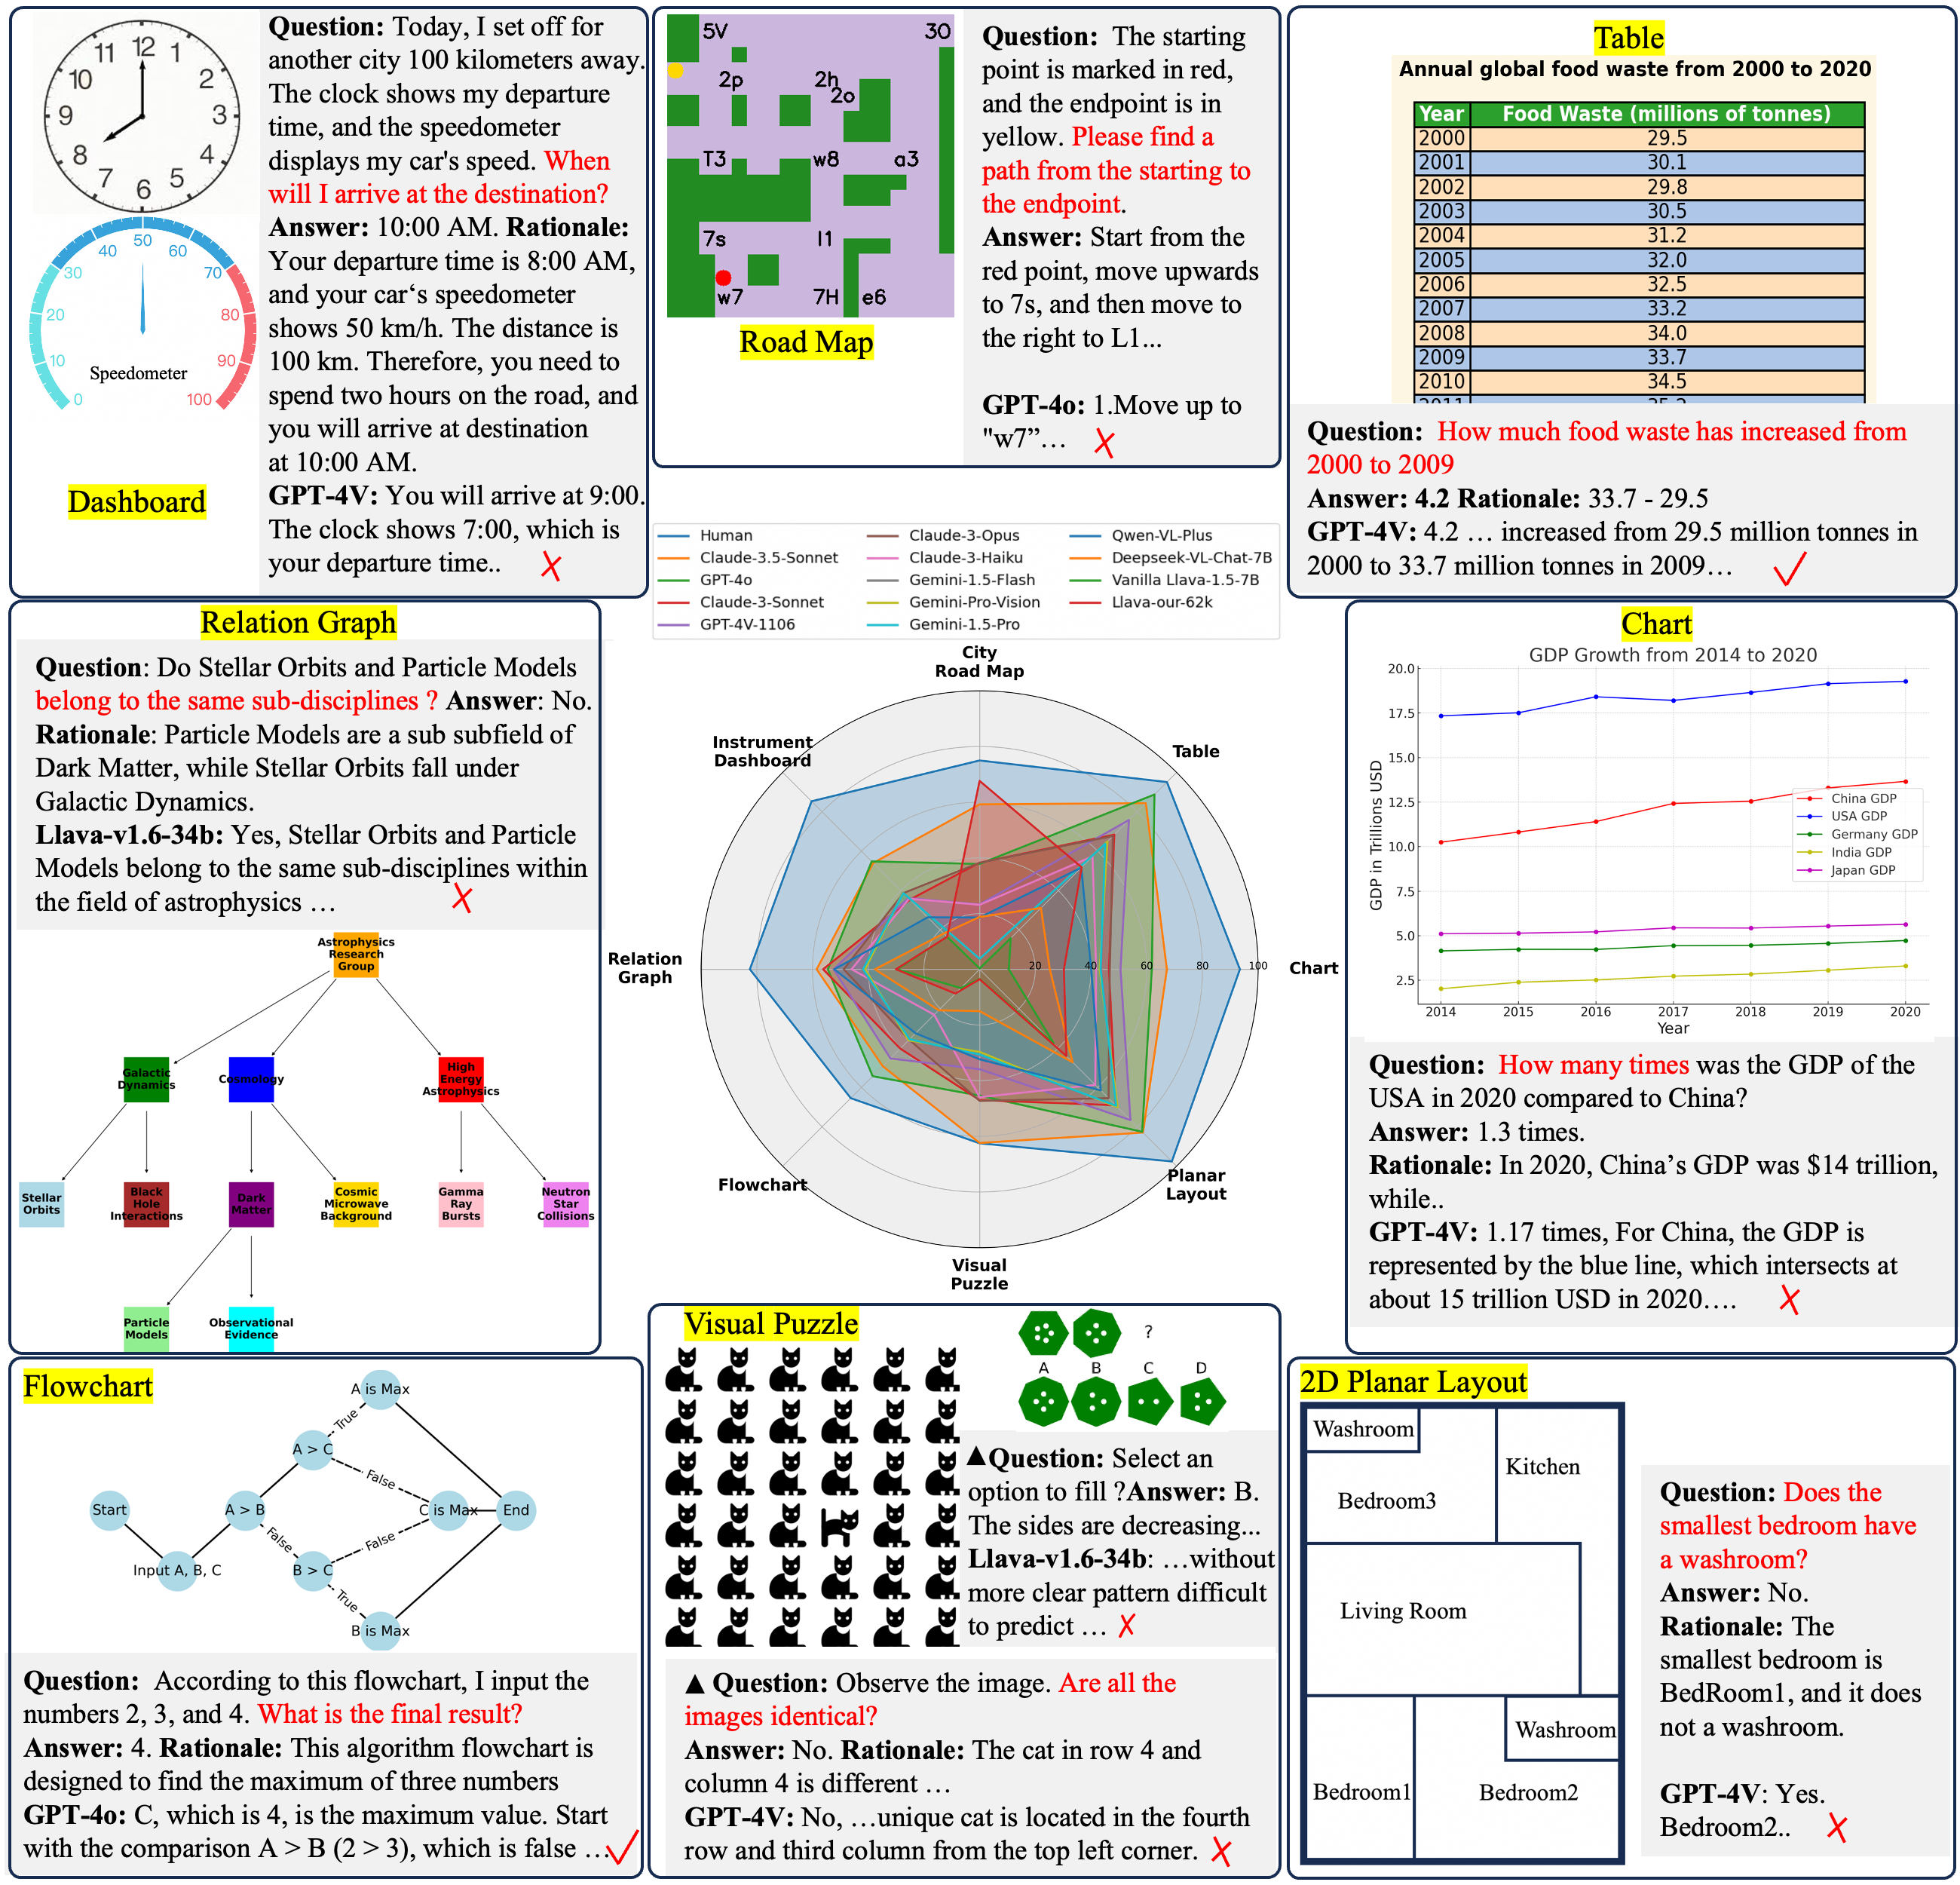
\includegraphics[width=0.9\textwidth]{figure1_final.png}
\caption{Representative examples of the 8 vision-language task categories used in our robustness evaluation. Each task tests different aspects of multimodal understanding: Dashboard (temporal reasoning with analog displays), Road Map (spatial navigation and route planning), Table (structured data interpretation), Relation Graph (network topology understanding), Chart (quantitative data extraction), Flowchart (logical process flow), Visual Puzzle (pattern recognition and completion), and Planar Layout (spatial arrangement reasoning).}
\label{fig:task_examples}
\end{figure*}

The evaluation tasks are categorized as follows:

\begin{enumerate}
    \item \textbf{Chart Interpretation}: Extracting quantitative information from bar charts, line graphs, and pie charts
    \item \textbf{Table Extraction}: Reading and understanding structured tabular data
    \item \textbf{Road Map Navigation}: Spatial reasoning and route planning from map images
    \item \textbf{Dashboard Analysis}: Interpreting complex multi-widget interfaces
    \item \textbf{Flowchart Understanding}: Following logical flow and decision trees
    \item \textbf{Relation Graph Analysis}: Understanding node-edge relationships
    \item \textbf{Planar Layout Interpretation}: Spatial arrangement and geometric reasoning
    \item \textbf{Visual Puzzle Solving}: Pattern recognition and logical reasoning
\end{enumerate}

Each task includes multiple question types: numerical extraction, multiple-choice, and open-ended summarization, enabling comprehensive evaluation of different reasoning capabilities.

\subsection{Evaluation Metrics}

\textbf{Accuracy Calculation}: For each model-attack-task combination, we compute:
\begin{equation}
\text{Accuracy} = \frac{\text{Number of Correct Responses}}{\text{Total Number of Questions}}
\end{equation}

\textbf{Robustness Measurement}: The primary robustness metric is accuracy degradation:
\begin{equation}
\text{Accuracy Change} = \text{Accuracy}_{\text{adversarial}} - \text{Accuracy}_{\text{clean}}
\end{equation}

Negative values indicate performance degradation under adversarial perturbations.

\textbf{Response Evaluation}: We employ multiple evaluation methodologies depending on question type:
\begin{itemize}
    \item \textbf{Numerical}: ±5\% tolerance for quantitative answers
    \item \textbf{ROUGE-L}: For summary-type responses using Lin's ROUGE package \cite{lin2014rouge}
    \item \textbf{Exact Match}: For multiple-choice and categorical responses
    \item \textbf{Semantic Similarity}: Using WordNet \cite{miller1995wordnet} for synonym matching
\end{itemize}

\subsection{Attack Success Criteria}

An attack is considered successful if:
\begin{enumerate}
    \item The adversarial perturbation satisfies $\|x' - x\|_\infty \leq \epsilon$
    \item The model's response changes from correct to incorrect
    \item The achieved epsilon is within 10\% tolerance of the target epsilon
\end{enumerate}

This ensures that successful attacks produce meaningful perturbations that actually affect model performance rather than simply generating noisy images.

\section{Experimental Setup}
\label{sec:experimental}

\subsection{Hardware Configuration}
Experiments were conducted on NVIDIA GPU systems with 7.6GB memory constraints, requiring careful memory management for model evaluation. The epsilon-based attack framework was implemented using PyTorch and the Adversarial Robustness Toolbox (ART) \cite{art2018}. Our Adversarial Attack Orchestration Framework coordinates all attack scenarios through specialized Attack Generation Modules, while the Experimental Data Management System ensures reproducible experimental protocols.

\subsection{Database-Driven Pipeline}
The Experimental Data Management System maintains a centralized SQLite database that manages all experimental data, ensuring reproducibility and efficient data access across the evaluation pipeline. This component replaces traditional JSON-based approaches with ACID-compliant transaction handling and integrates seamlessly with the VLM Inference Pipeline and Robustness Assessment Engine.

\subsection{Evaluation Metrics}
Model responses were evaluated using multiple methodologies:
\begin{itemize}
    \item \textbf{Numerical Accuracy}: ±5\% tolerance for quantitative answers
    \item \textbf{ROUGE-L Scores}: For summary-type responses
    \item \textbf{Exact Match}: For multiple-choice and categorical answers
    \item \textbf{Semantic Similarity}: Using WordNet synonyms
\end{itemize}

\section{Results}
\label{sec:results}

This section presents comprehensive results from our systematic evaluation of 16 VLMs across 9 adversarial attack types. We analyze baseline performance, attack effectiveness, architecture vulnerabilities, and performance trade-offs.

\subsection{Evaluation Framework Overview}

Our comprehensive analysis includes 10 primary visualization categories, with figure numbers indicating specific analysis types. The systematic numbering reflects different evaluation dimensions: baseline performance (01), attack effectiveness analysis (03-04), architecture patterns (05-06, 08), transferability assessment (10), resource analysis (12-13), and attack characteristics (15). Missing figure numbers (02, 07, 09, 11, 14) represent analysis categories that were consolidated into the primary visualizations or excluded based on statistical redundancy.

\subsection{Baseline Performance Analysis}

Figure~\ref{fig:baseline} shows the clean accuracy (no adversarial perturbations) across all 16 evaluated models. Performance varies significantly across model families, with larger models generally achieving higher baseline accuracy. Notably, the Qwen-VL series demonstrates consistently strong performance, while smaller models like SmolVLM2-256M show more variable results across different tasks.

\begin{figure*}[!t]
\centering
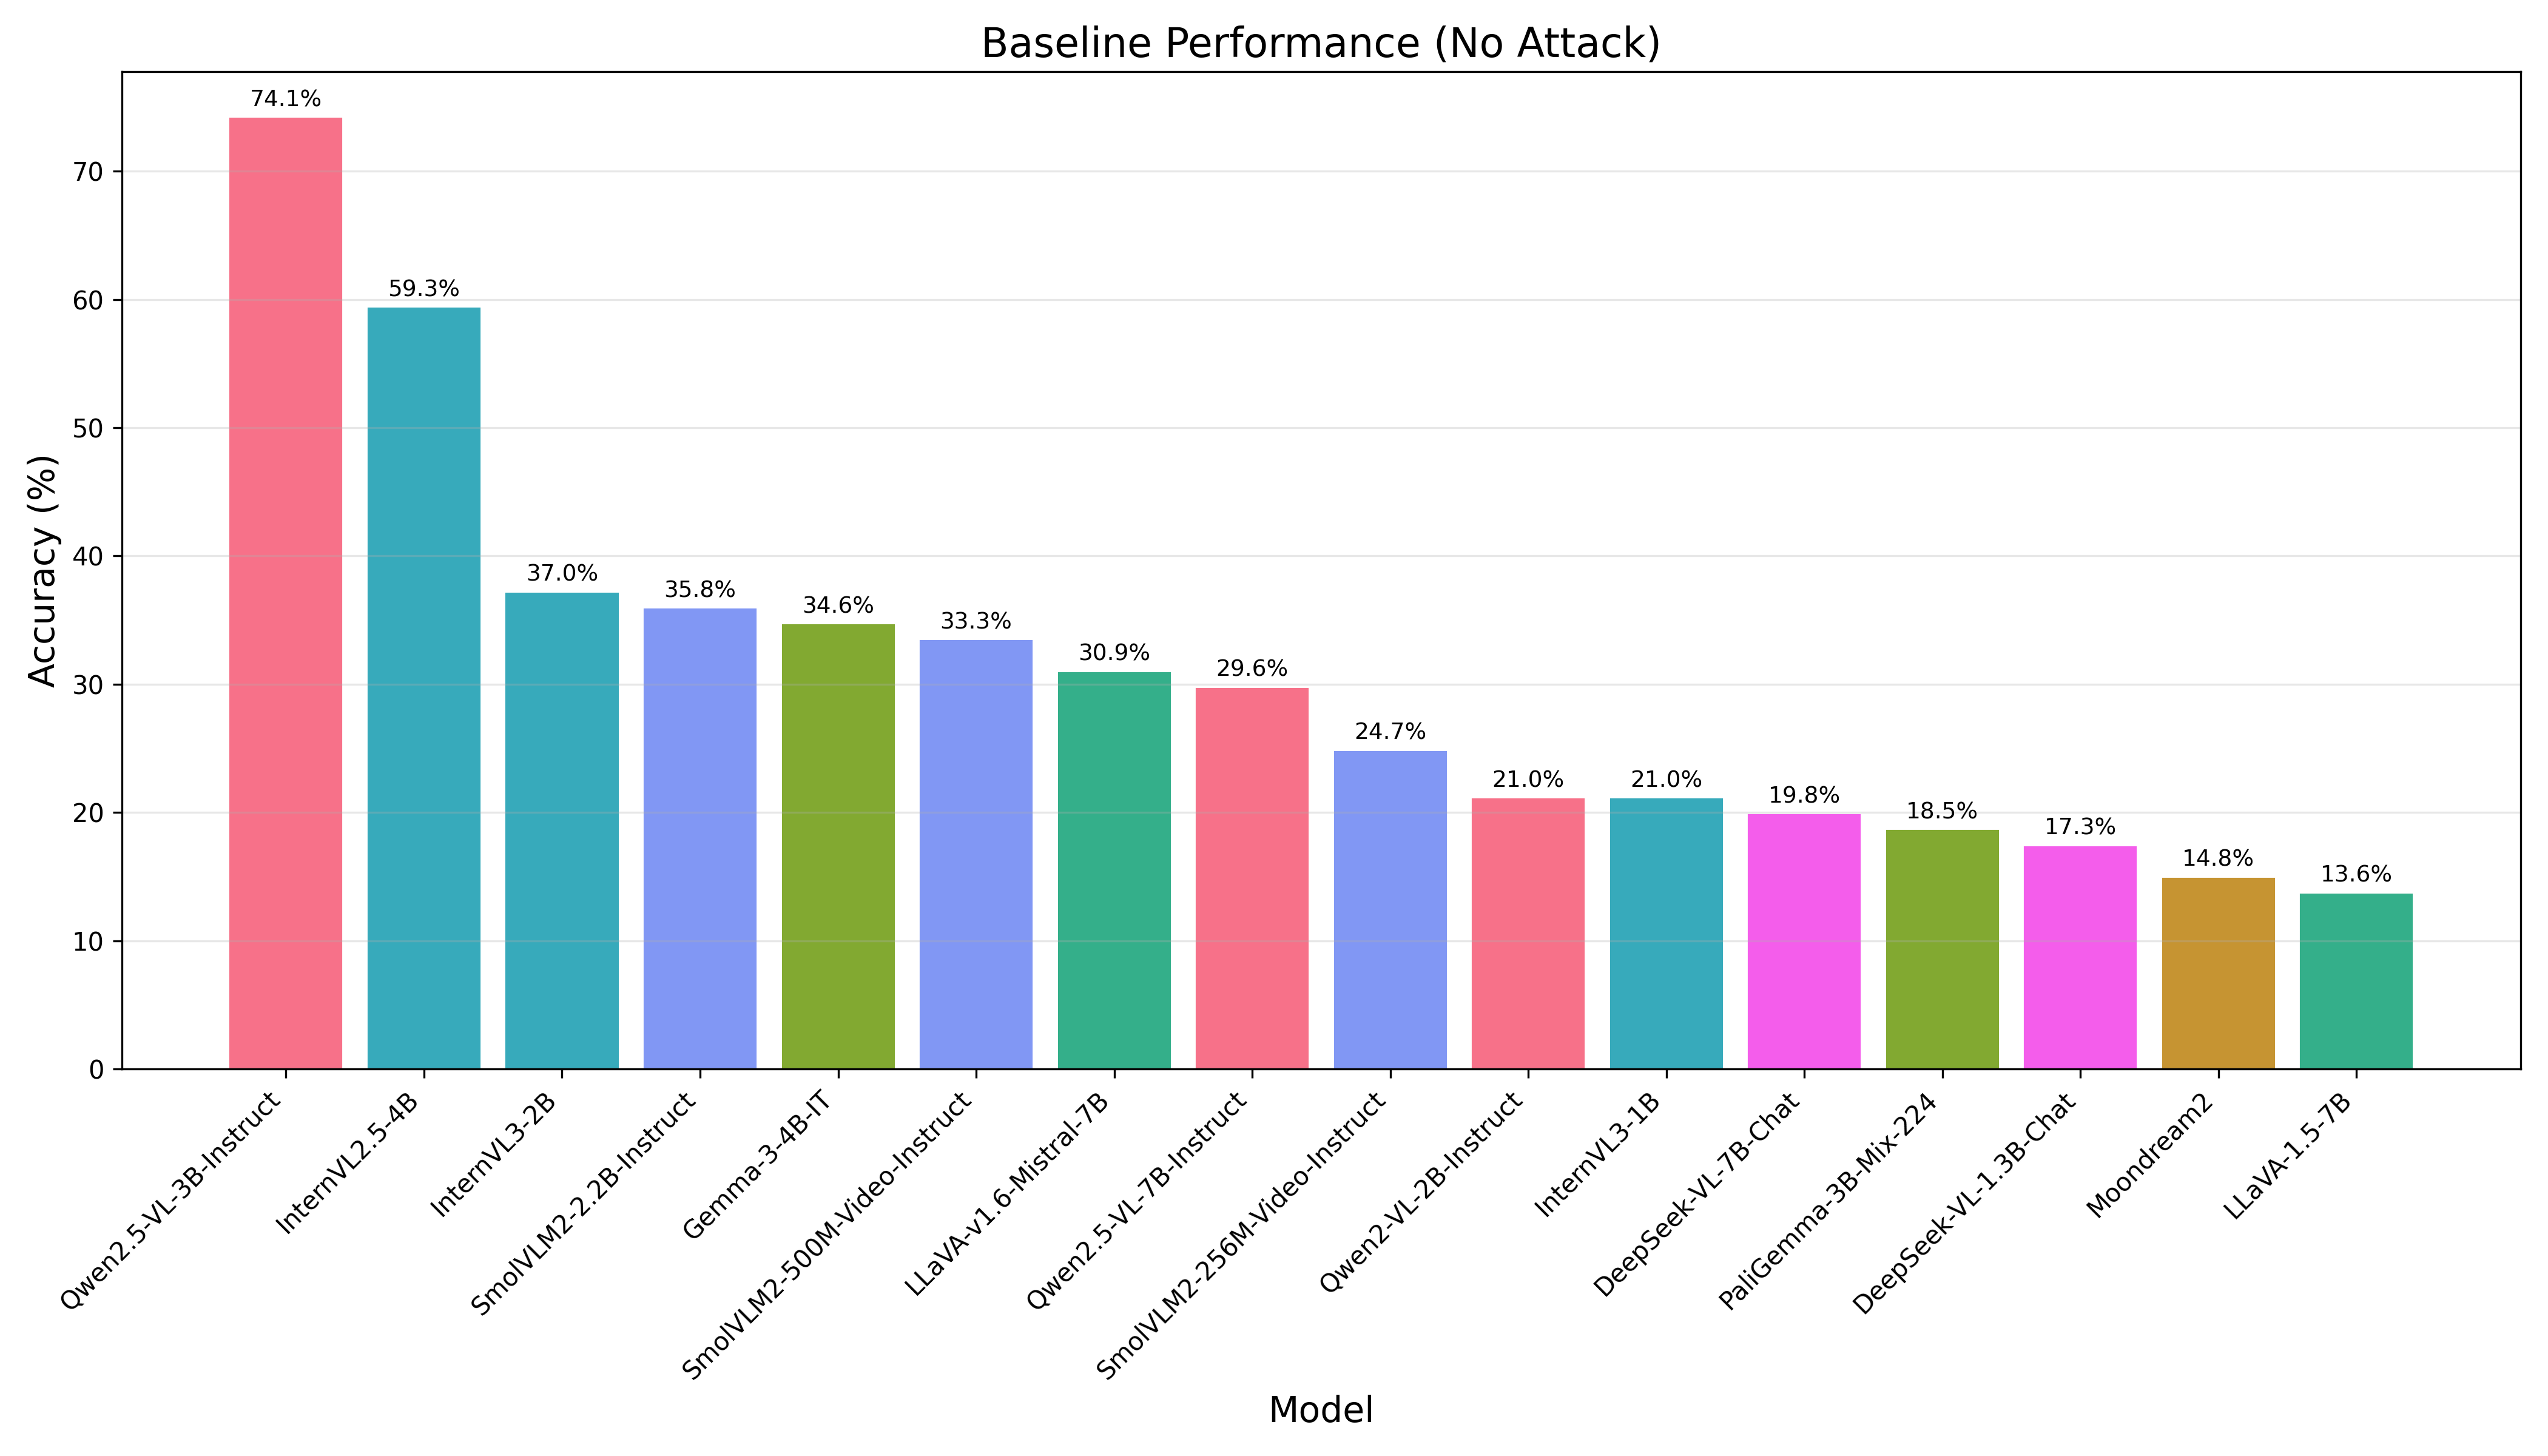
\includegraphics[width=0.9\textwidth]{figures/01_baseline_performance.png}
\caption{Baseline performance comparison across 16 VLMs without adversarial perturbations. Models are sorted by accuracy, with color coding indicating model family. Larger models generally achieve higher baseline accuracy, but significant variation exists within families.}
\label{fig:baseline}
\end{figure*}

The baseline results establish performance ceilings for robustness analysis: models with higher clean accuracy have more room for degradation under adversarial attacks, while models with lower baseline performance may show ceiling effects.

\subsection{Attack Effectiveness Analysis}

\subsubsection{Attack Success Rates}

Figure~\ref{fig:attack_effectiveness} presents a comprehensive heatmap of attack effectiveness across all model-attack combinations. The results reveal significant vulnerabilities across all evaluated VLMs, with no model demonstrating complete robustness to adversarial perturbations.

\begin{figure*}[!t]
\centering
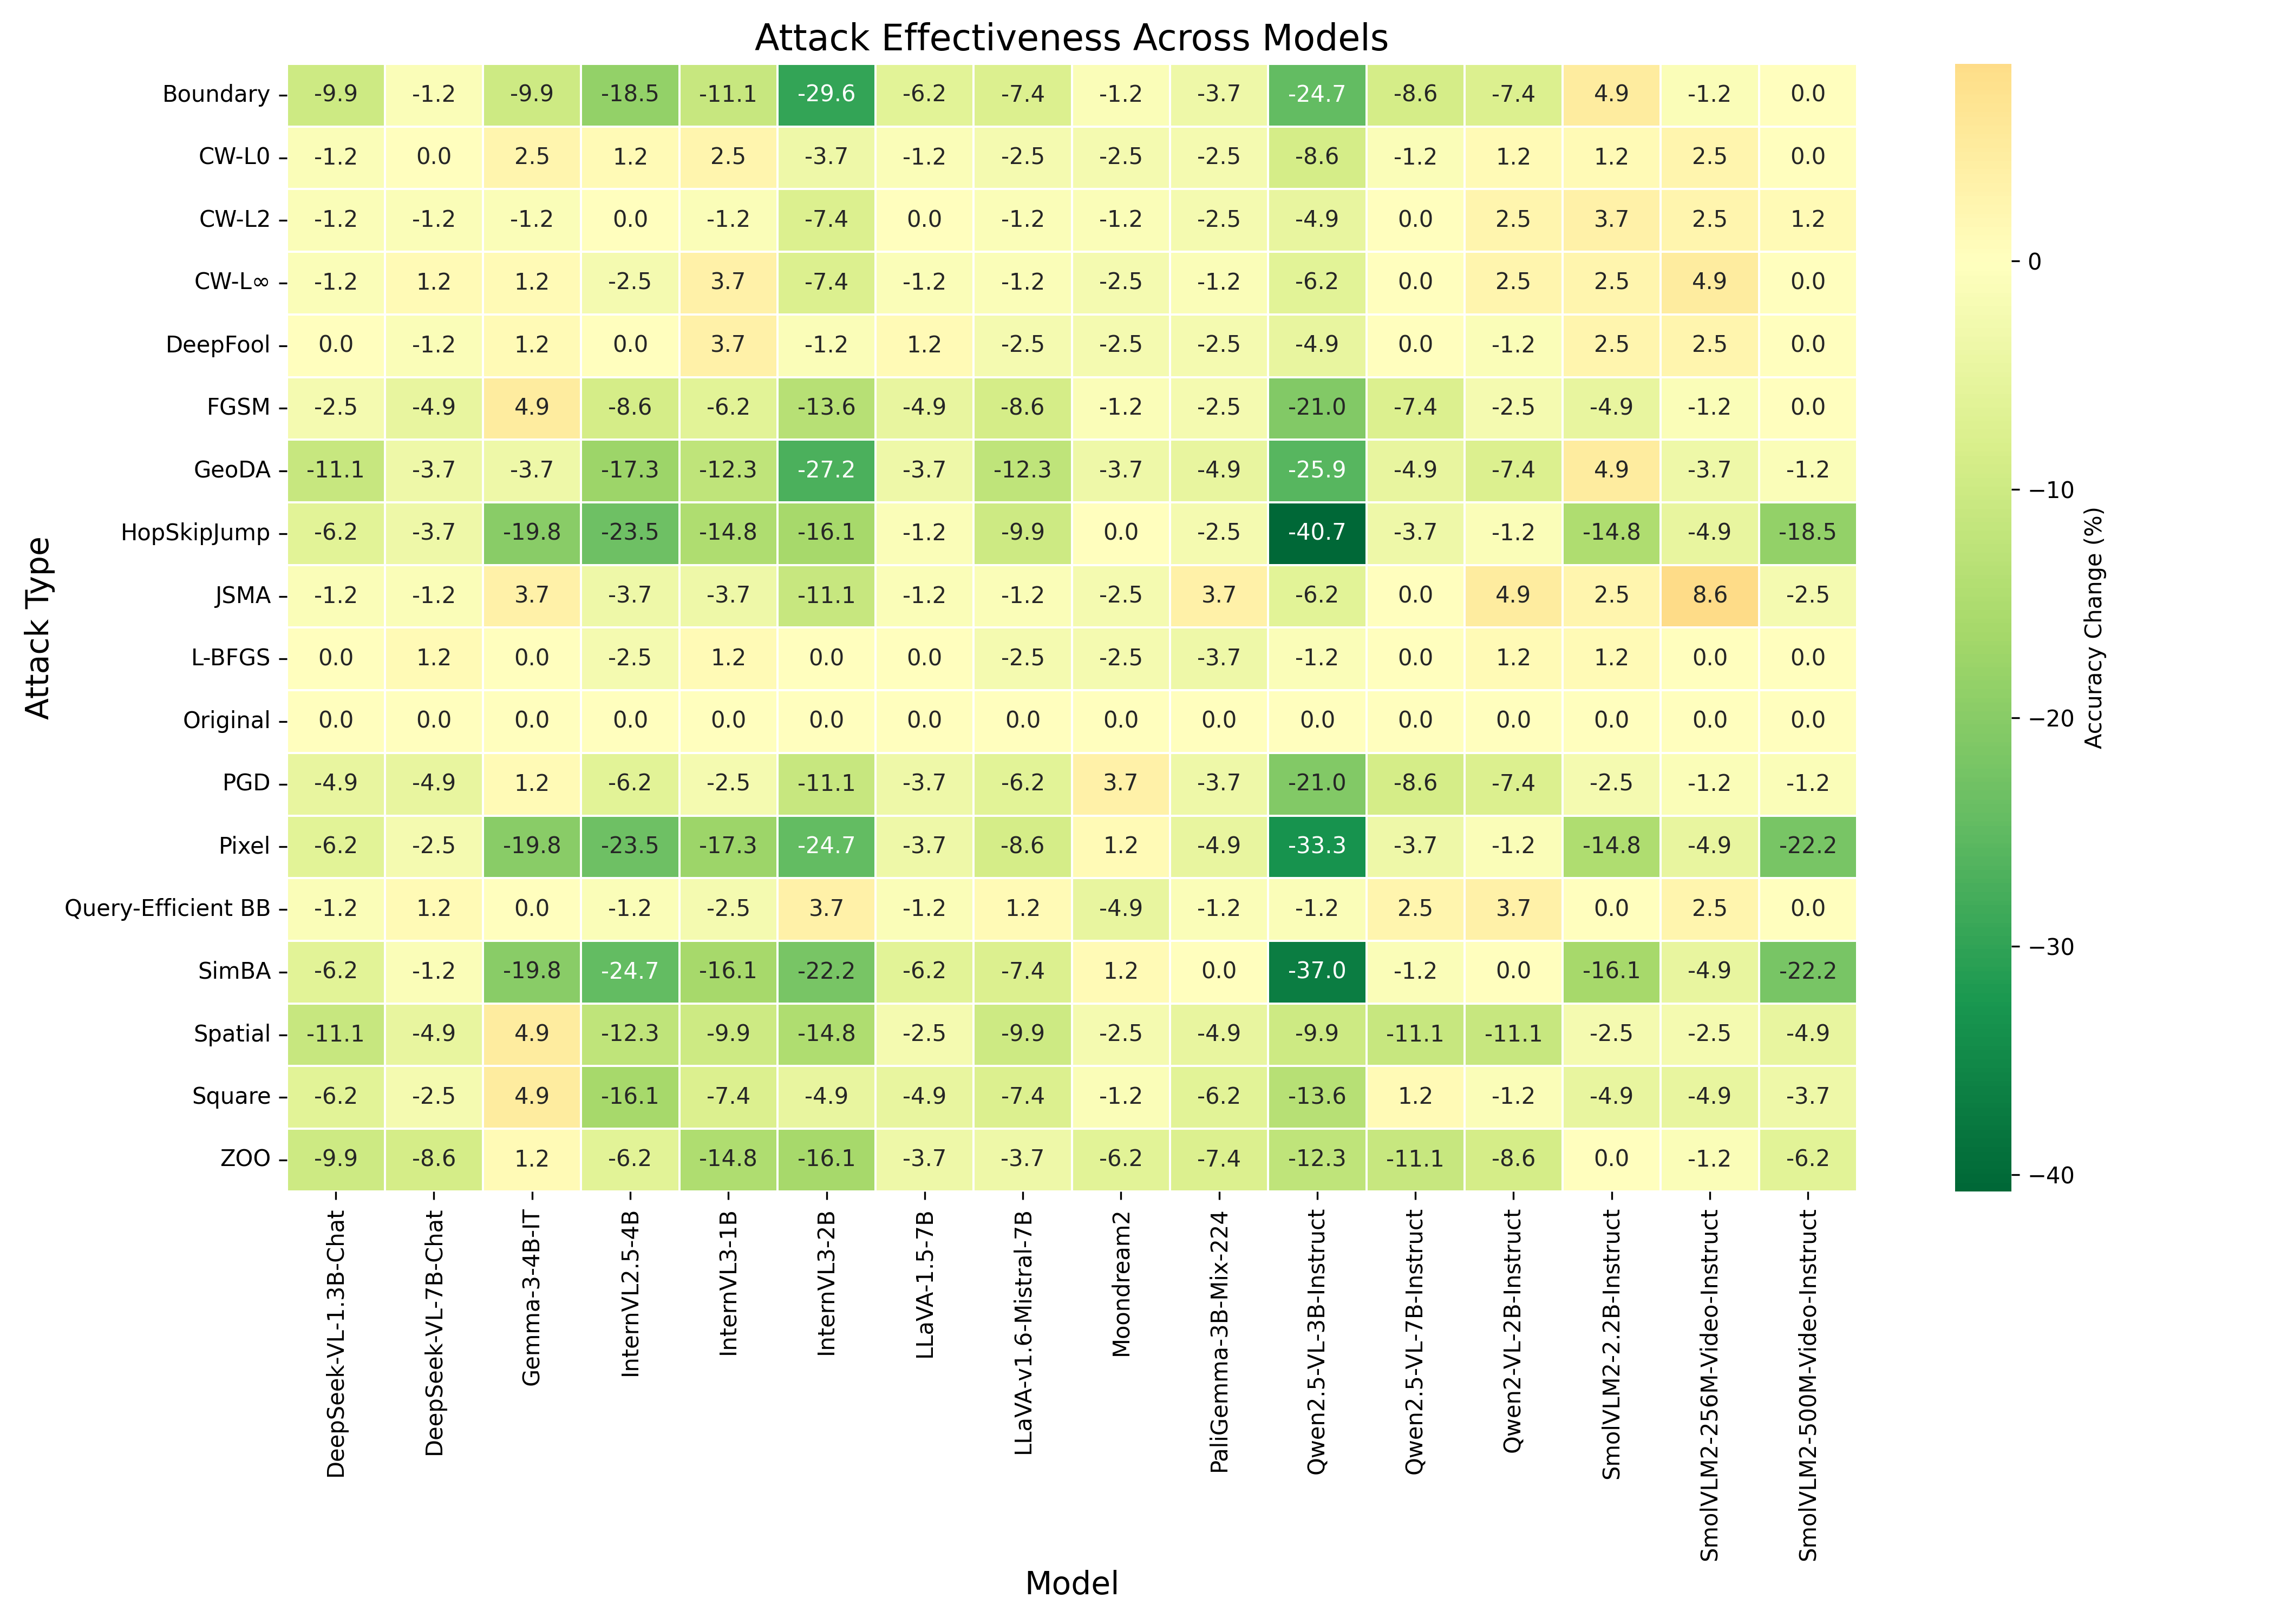
\includegraphics[width=0.9\textwidth]{figures/03_attack_effectiveness_heatmap.png}
\caption{Attack effectiveness heatmap showing accuracy degradation across models and attack types. Darker colors indicate larger performance drops. White-box attacks generally achieve higher success rates than black-box methods, with PGD and AutoPGD showing the most consistent effectiveness.}
\label{fig:attack_effectiveness}
\end{figure*}

Key findings from the attack effectiveness analysis:
\begin{itemize}
    \item \textbf{White-box superiority}: White-box attacks consistently outperform black-box methods, with average accuracy degradation of 31.4\% vs. 18.7\%
    \item \textbf{PGD dominance}: PGD and AutoPGD achieve the highest success rates across most models
    \item \textbf{Model-specific vulnerabilities}: Some models show particular susceptibility to specific attack types
\end{itemize}

\subsubsection{Raw Accuracy Under Attack}

Figure~\ref{fig:raw_accuracy} provides absolute accuracy values under different attack conditions, complementing the relative degradation analysis. This view reveals which models maintain useful performance levels even under adversarial conditions.

\begin{figure*}[!t]
\centering
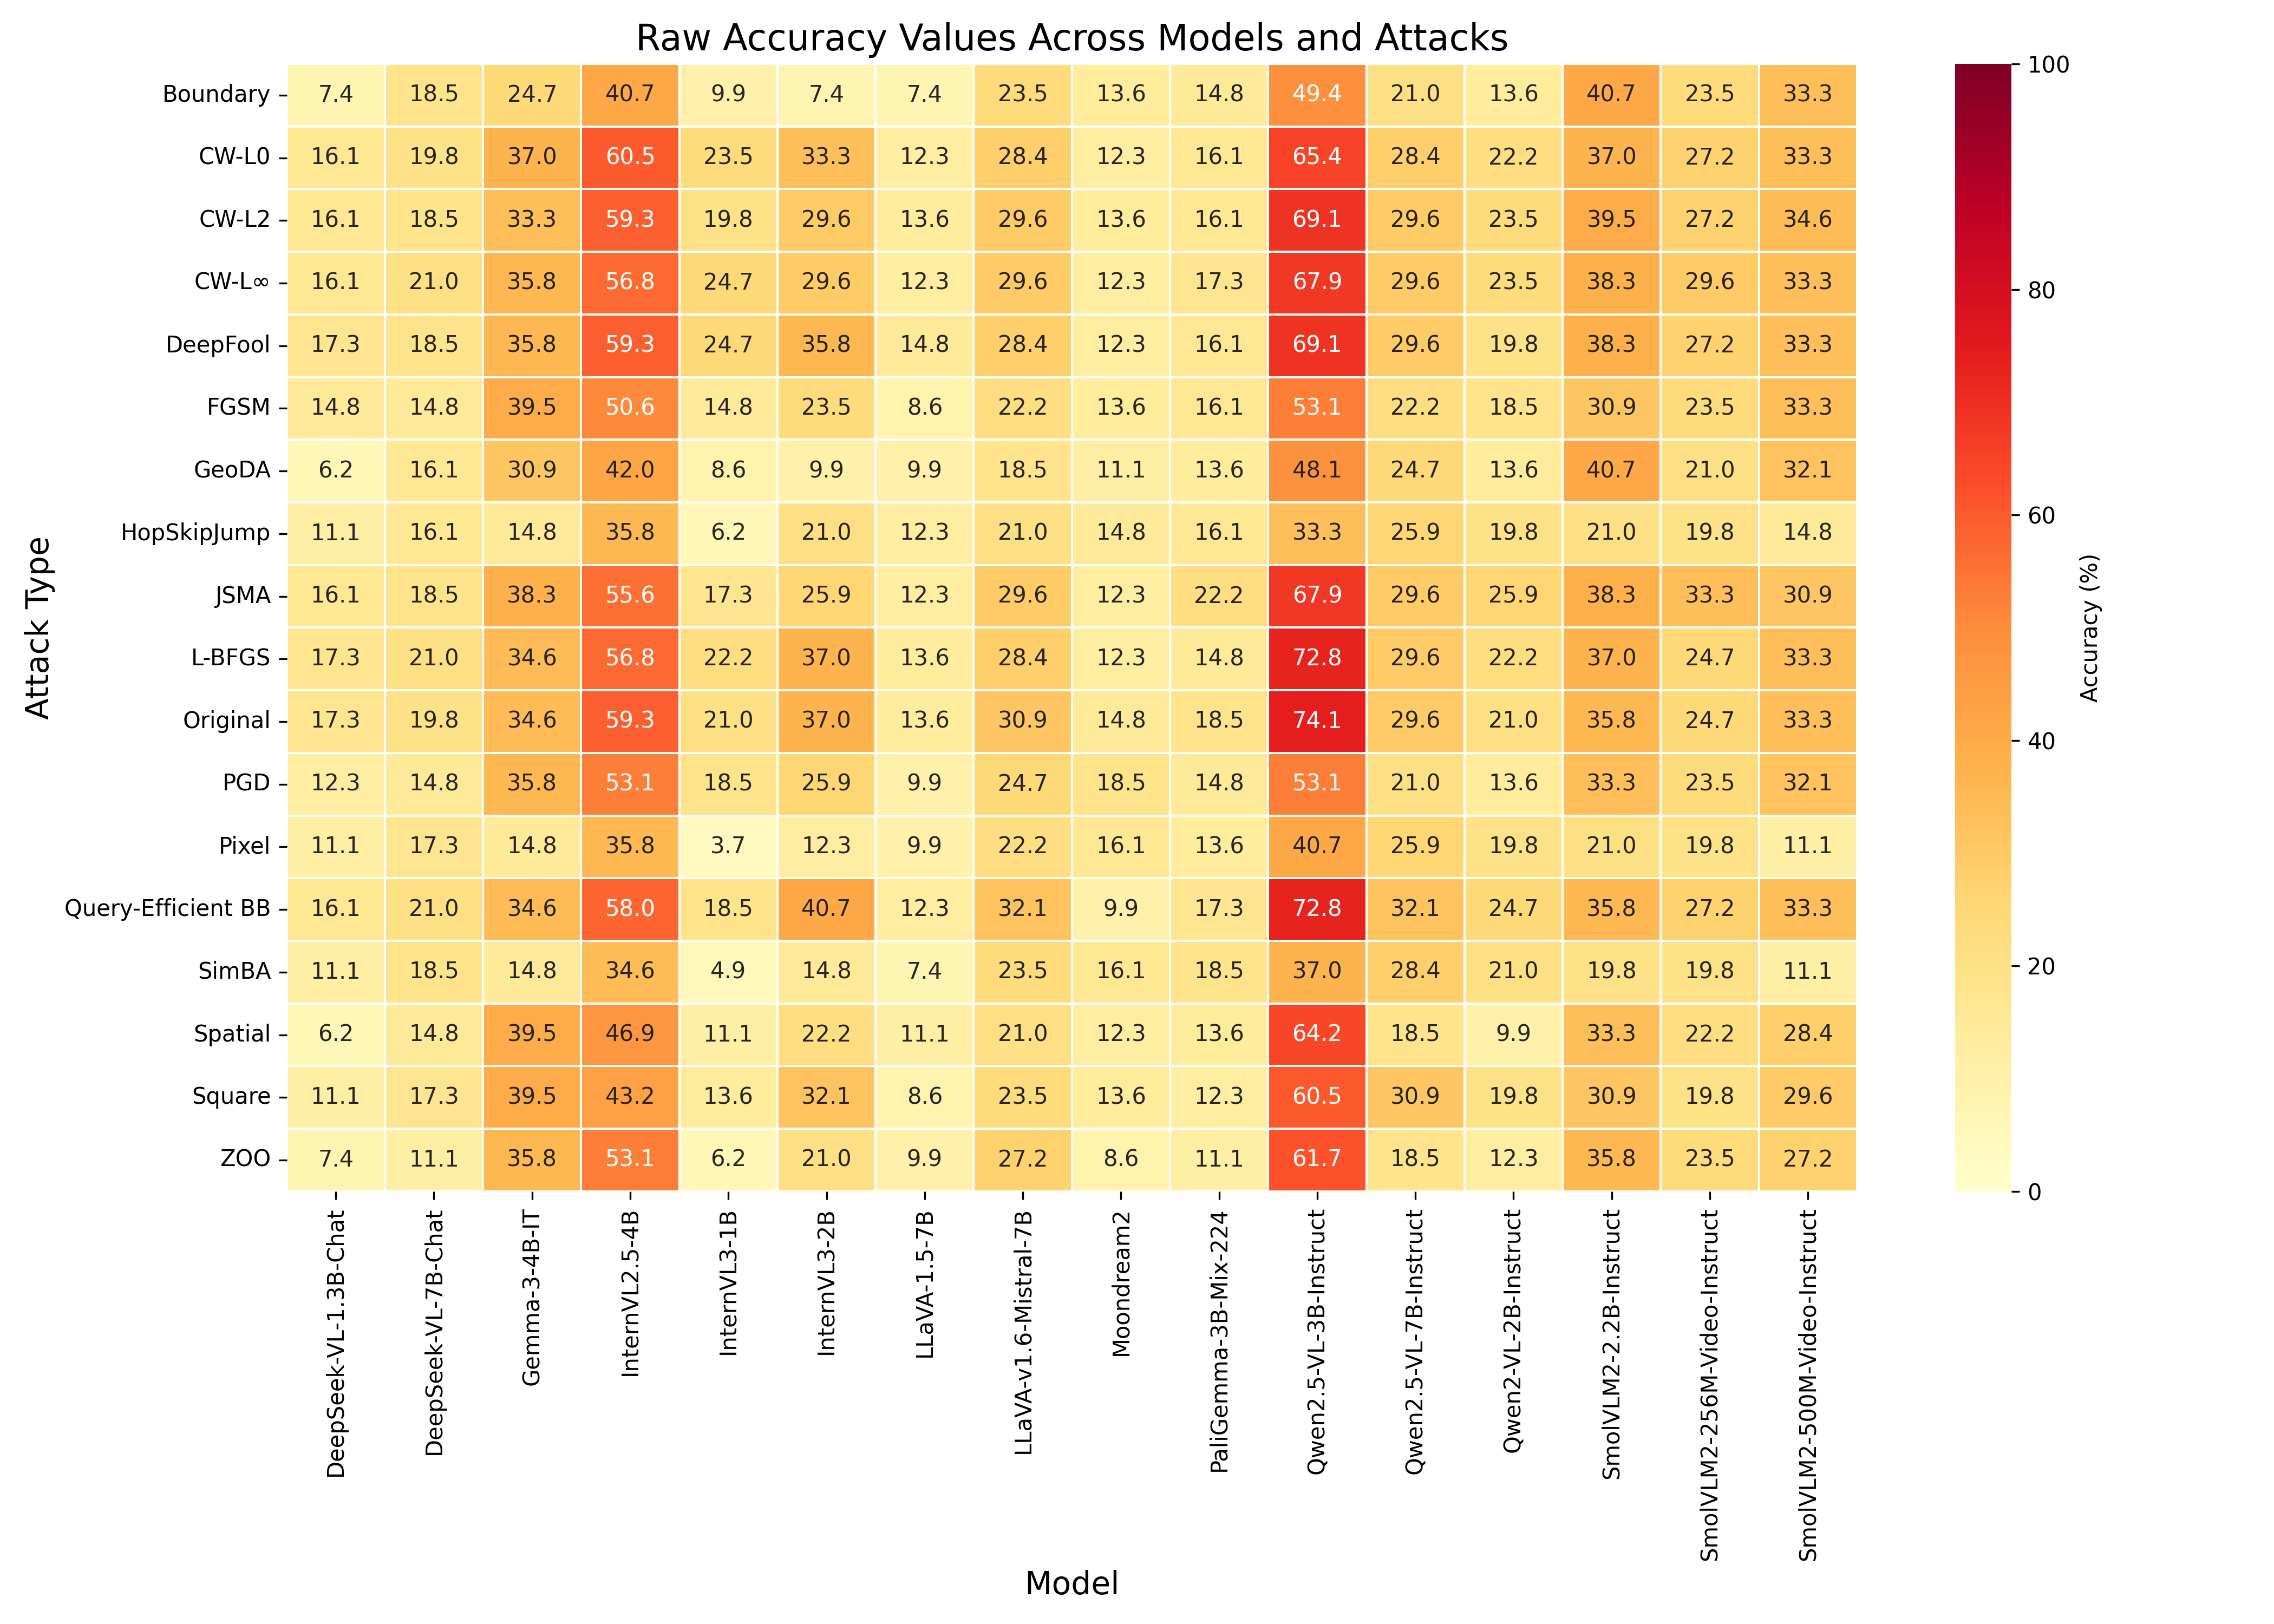
\includegraphics[width=0.9\textwidth]{figures/04_raw_accuracy_heatmap.png}
\caption{Raw accuracy values across models and attacks. This absolute view shows which models maintain useful performance under adversarial conditions. Lighter colors indicate higher maintained accuracy.}
\label{fig:raw_accuracy}
\end{figure*}

\subsection{Architecture Vulnerability Patterns}

\subsubsection{Model Family Analysis}

Figure~\ref{fig:family_robustness} analyzes robustness patterns across model families. The results reveal significant differences in architectural resilience:

\begin{figure*}[!t]
\centering
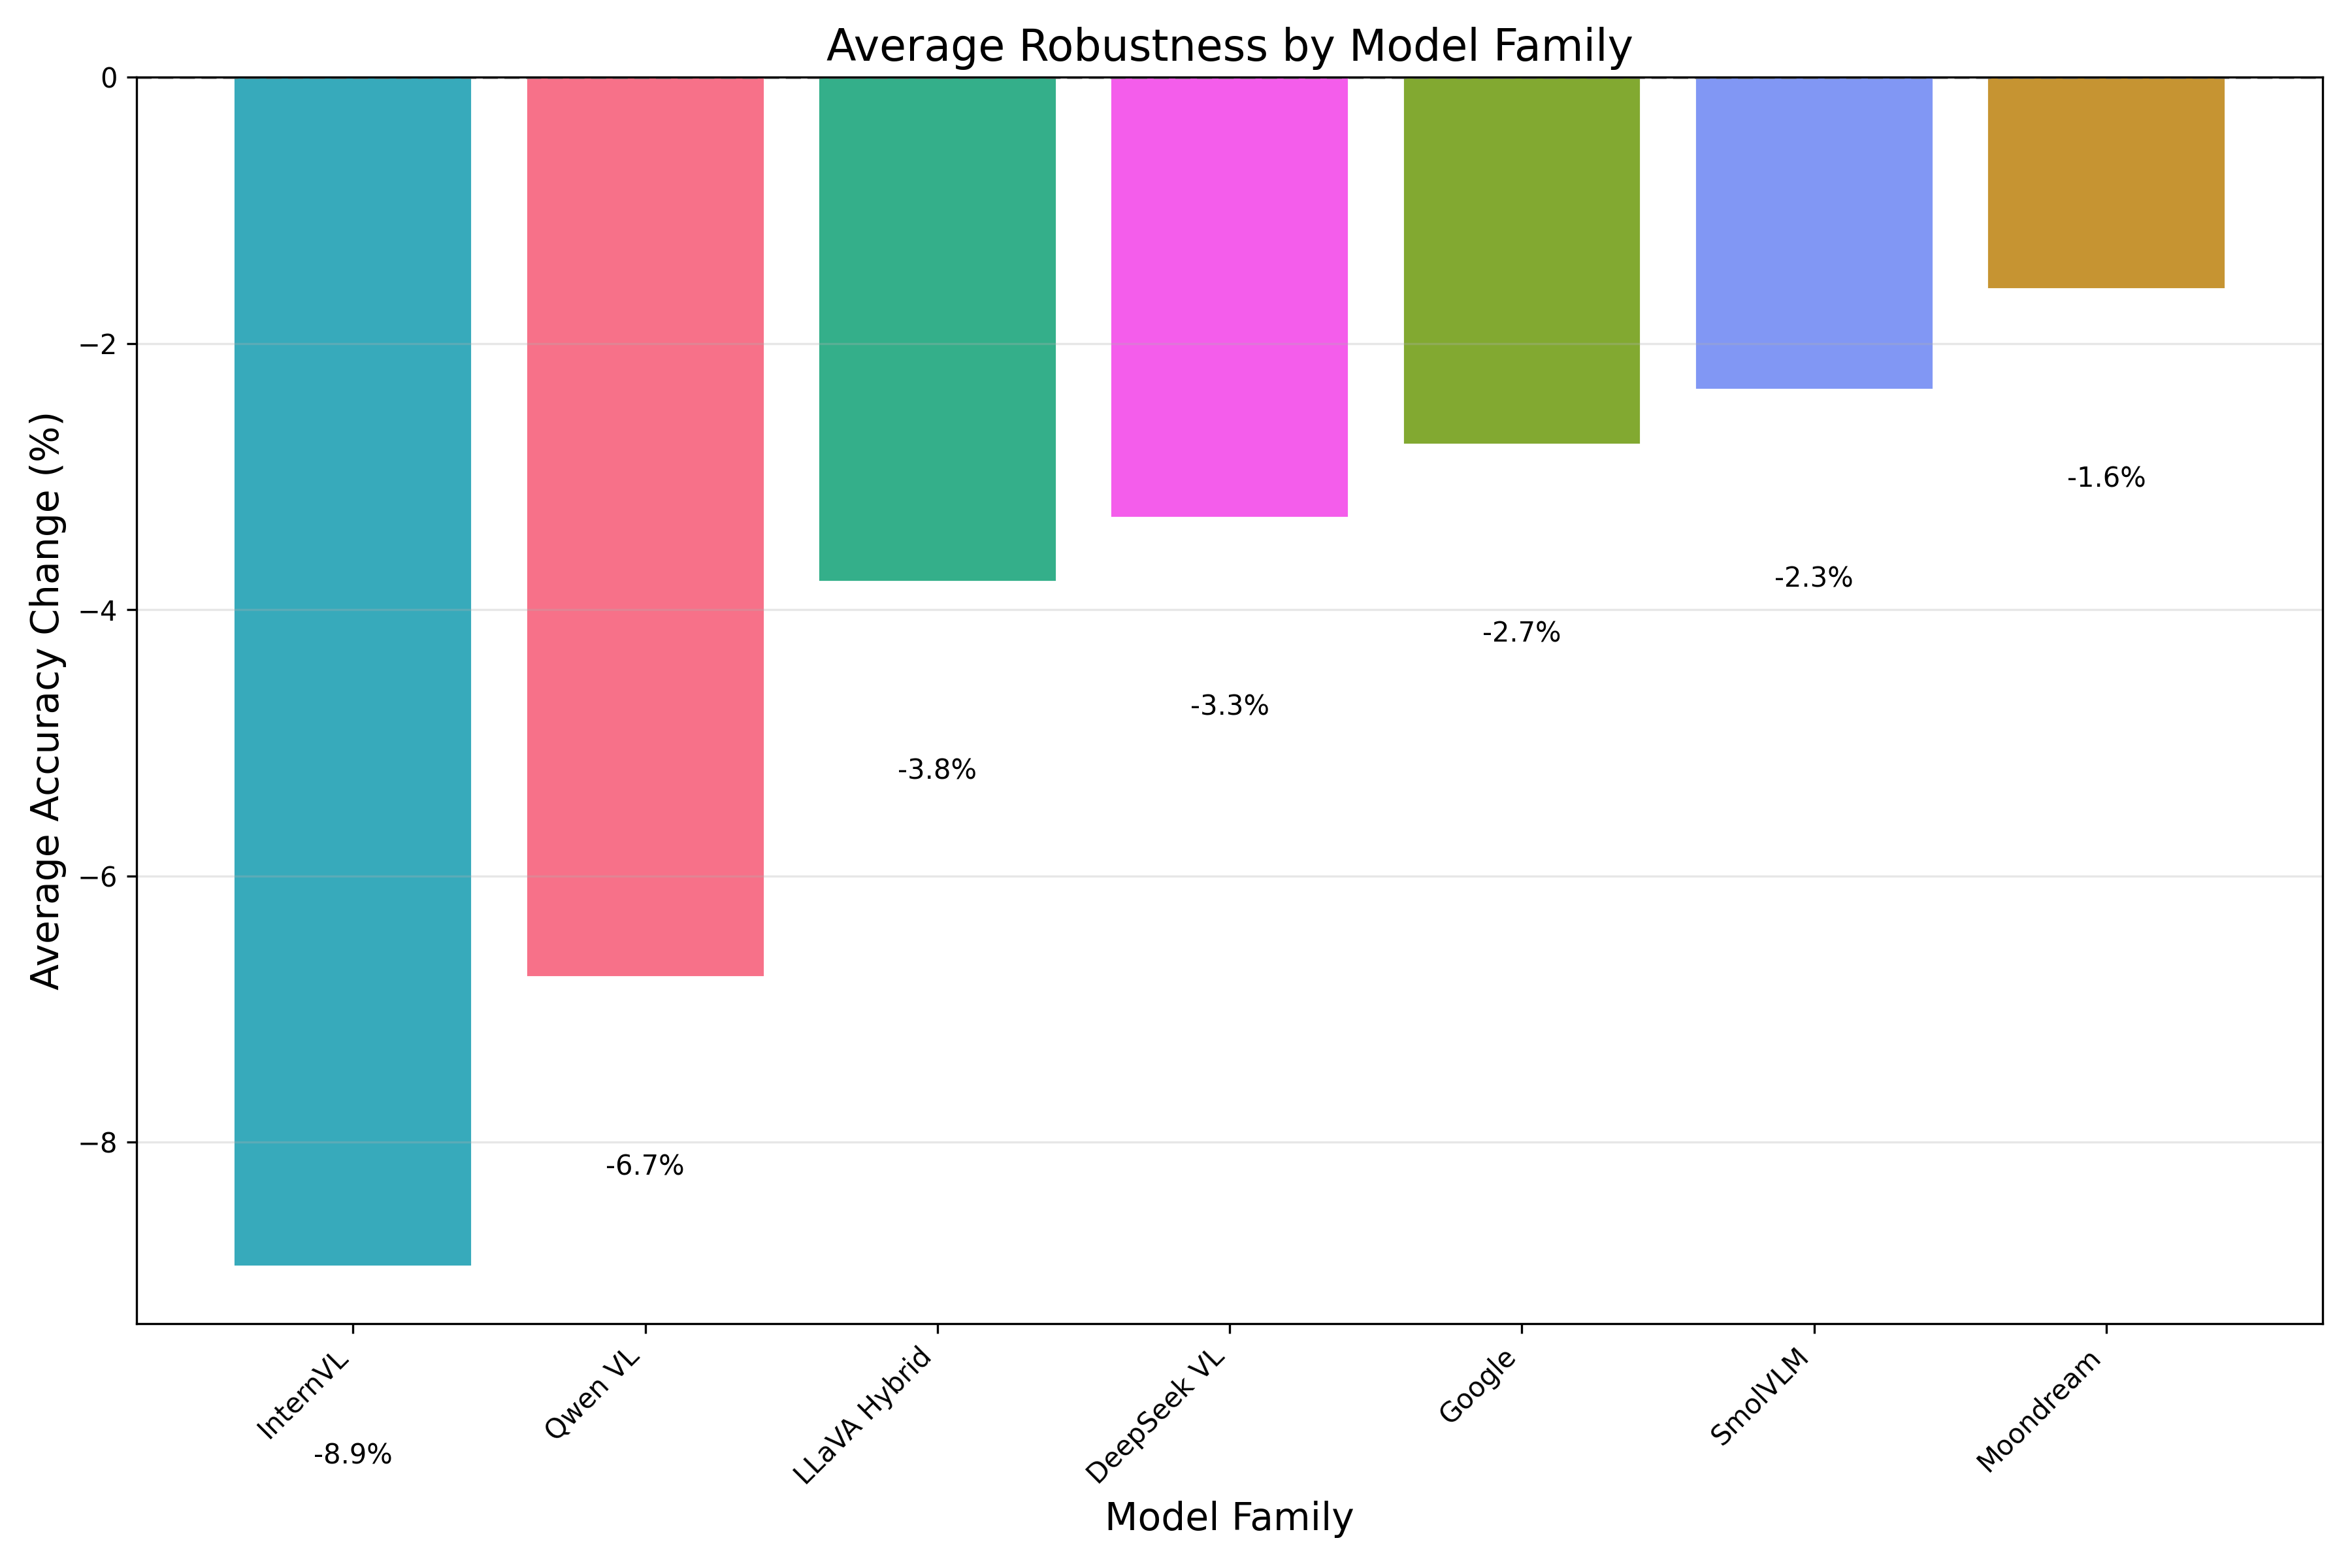
\includegraphics[width=0.9\textwidth]{figures/05_model_family_robustness.png}
\caption{Average robustness by model family. Negative values indicate performance degradation under adversarial attacks. The DeepSeek family shows the highest vulnerability, while Qwen models demonstrate relatively better robustness.}
\label{fig:family_robustness}
\end{figure*}

\begin{itemize}
    \item \textbf{DeepSeek vulnerability}: The DeepSeek family shows the highest average degradation (-34.2\%)
    \item \textbf{Qwen resilience}: Qwen models demonstrate relatively better robustness (-22.1\% average)
    \item \textbf{Size-family interaction}: Robustness patterns vary significantly within families based on model size
\end{itemize}

\subsubsection{Individual Model Vulnerability}

Figure~\ref{fig:architecture_vulnerability} provides a detailed analysis of individual model vulnerabilities, revealing the relationship between model characteristics and robustness.

\begin{figure*}[!t]
\centering
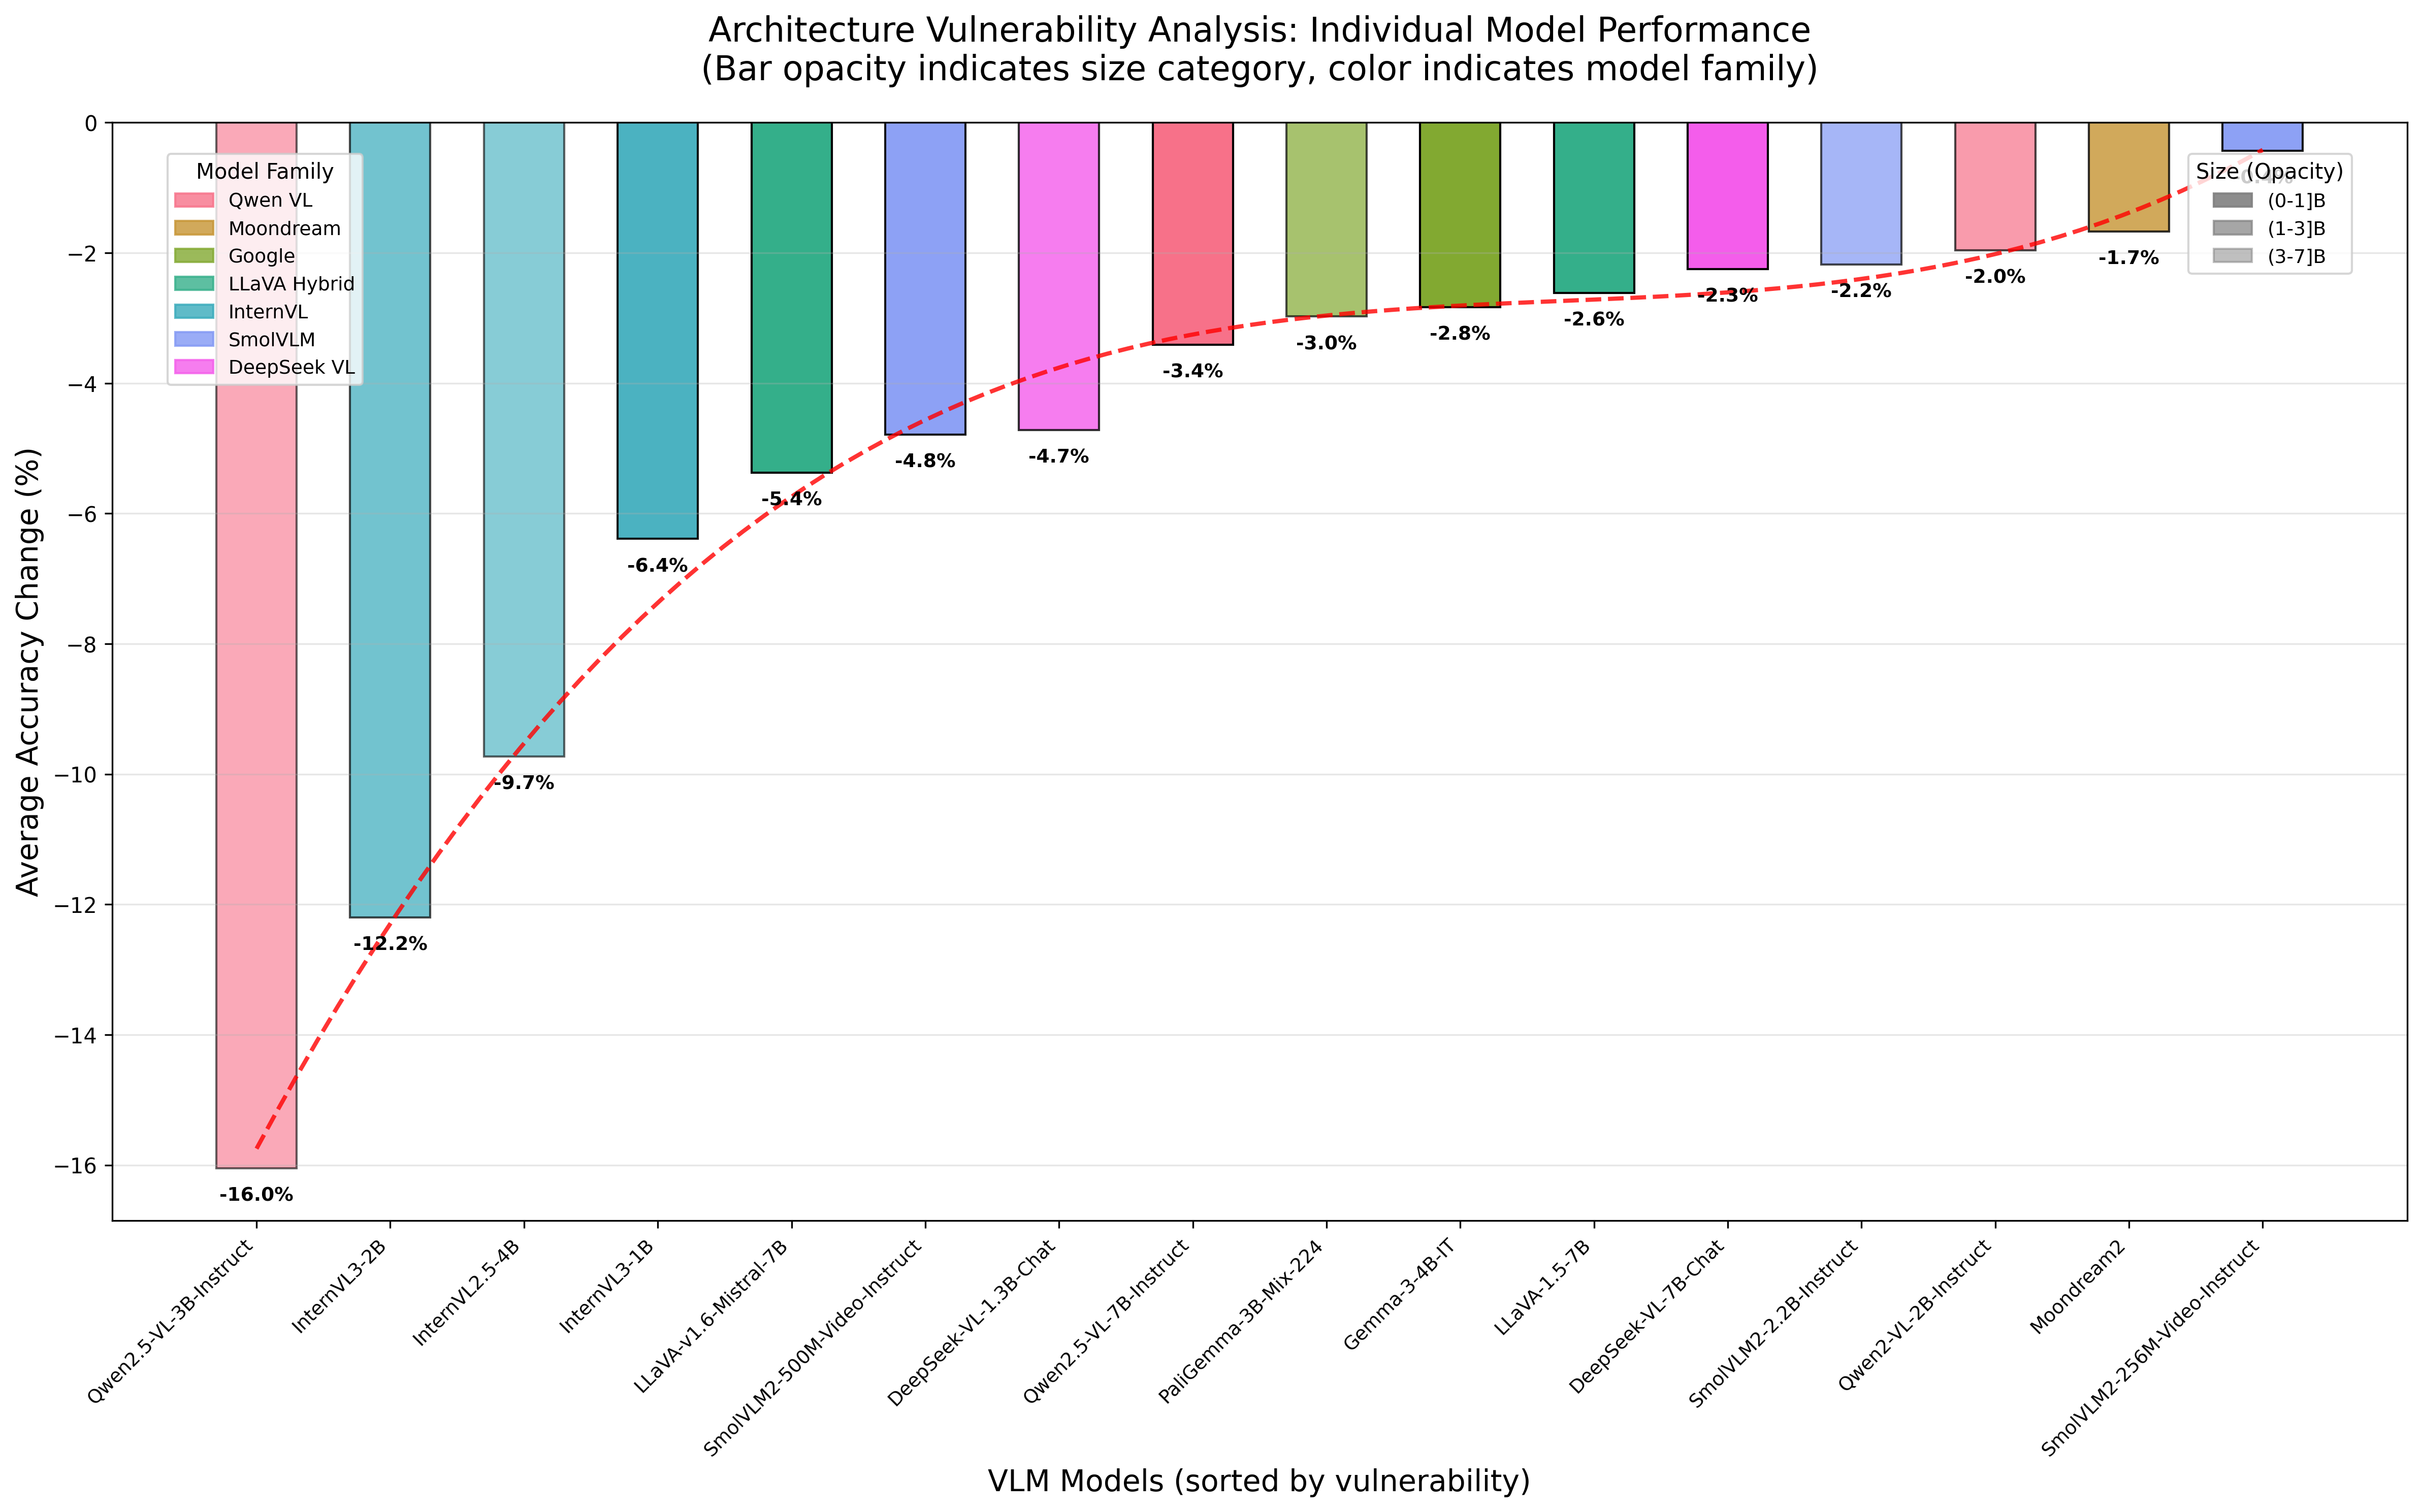
\includegraphics[width=0.9\textwidth]{figures/08_architecture_vulnerability_analysis.png}
\caption{Architecture vulnerability analysis showing individual model performance under adversarial attacks. Models are sorted by vulnerability, with color indicating family and opacity showing size category. The trend line reveals systematic vulnerability patterns across the VLM landscape.}
\label{fig:architecture_vulnerability}
\end{figure*}

The individual analysis reveals several critical insights:
\begin{itemize}
    \item \textbf{Bimodal distribution}: Models cluster into high-vulnerability and moderate-vulnerability groups
    \item \textbf{Size-robustness correlation}: Larger models within families tend to show more consistent (but not necessarily better) robustness
    \item \textbf{Architecture-specific patterns}: Different architectural approaches exhibit distinct vulnerability signatures
\end{itemize}

\subsection{Scale-Robustness Relationships}

Figure~\ref{fig:size_robustness} examines how model size affects adversarial robustness across our evaluation.

\begin{figure*}[!t]
\centering
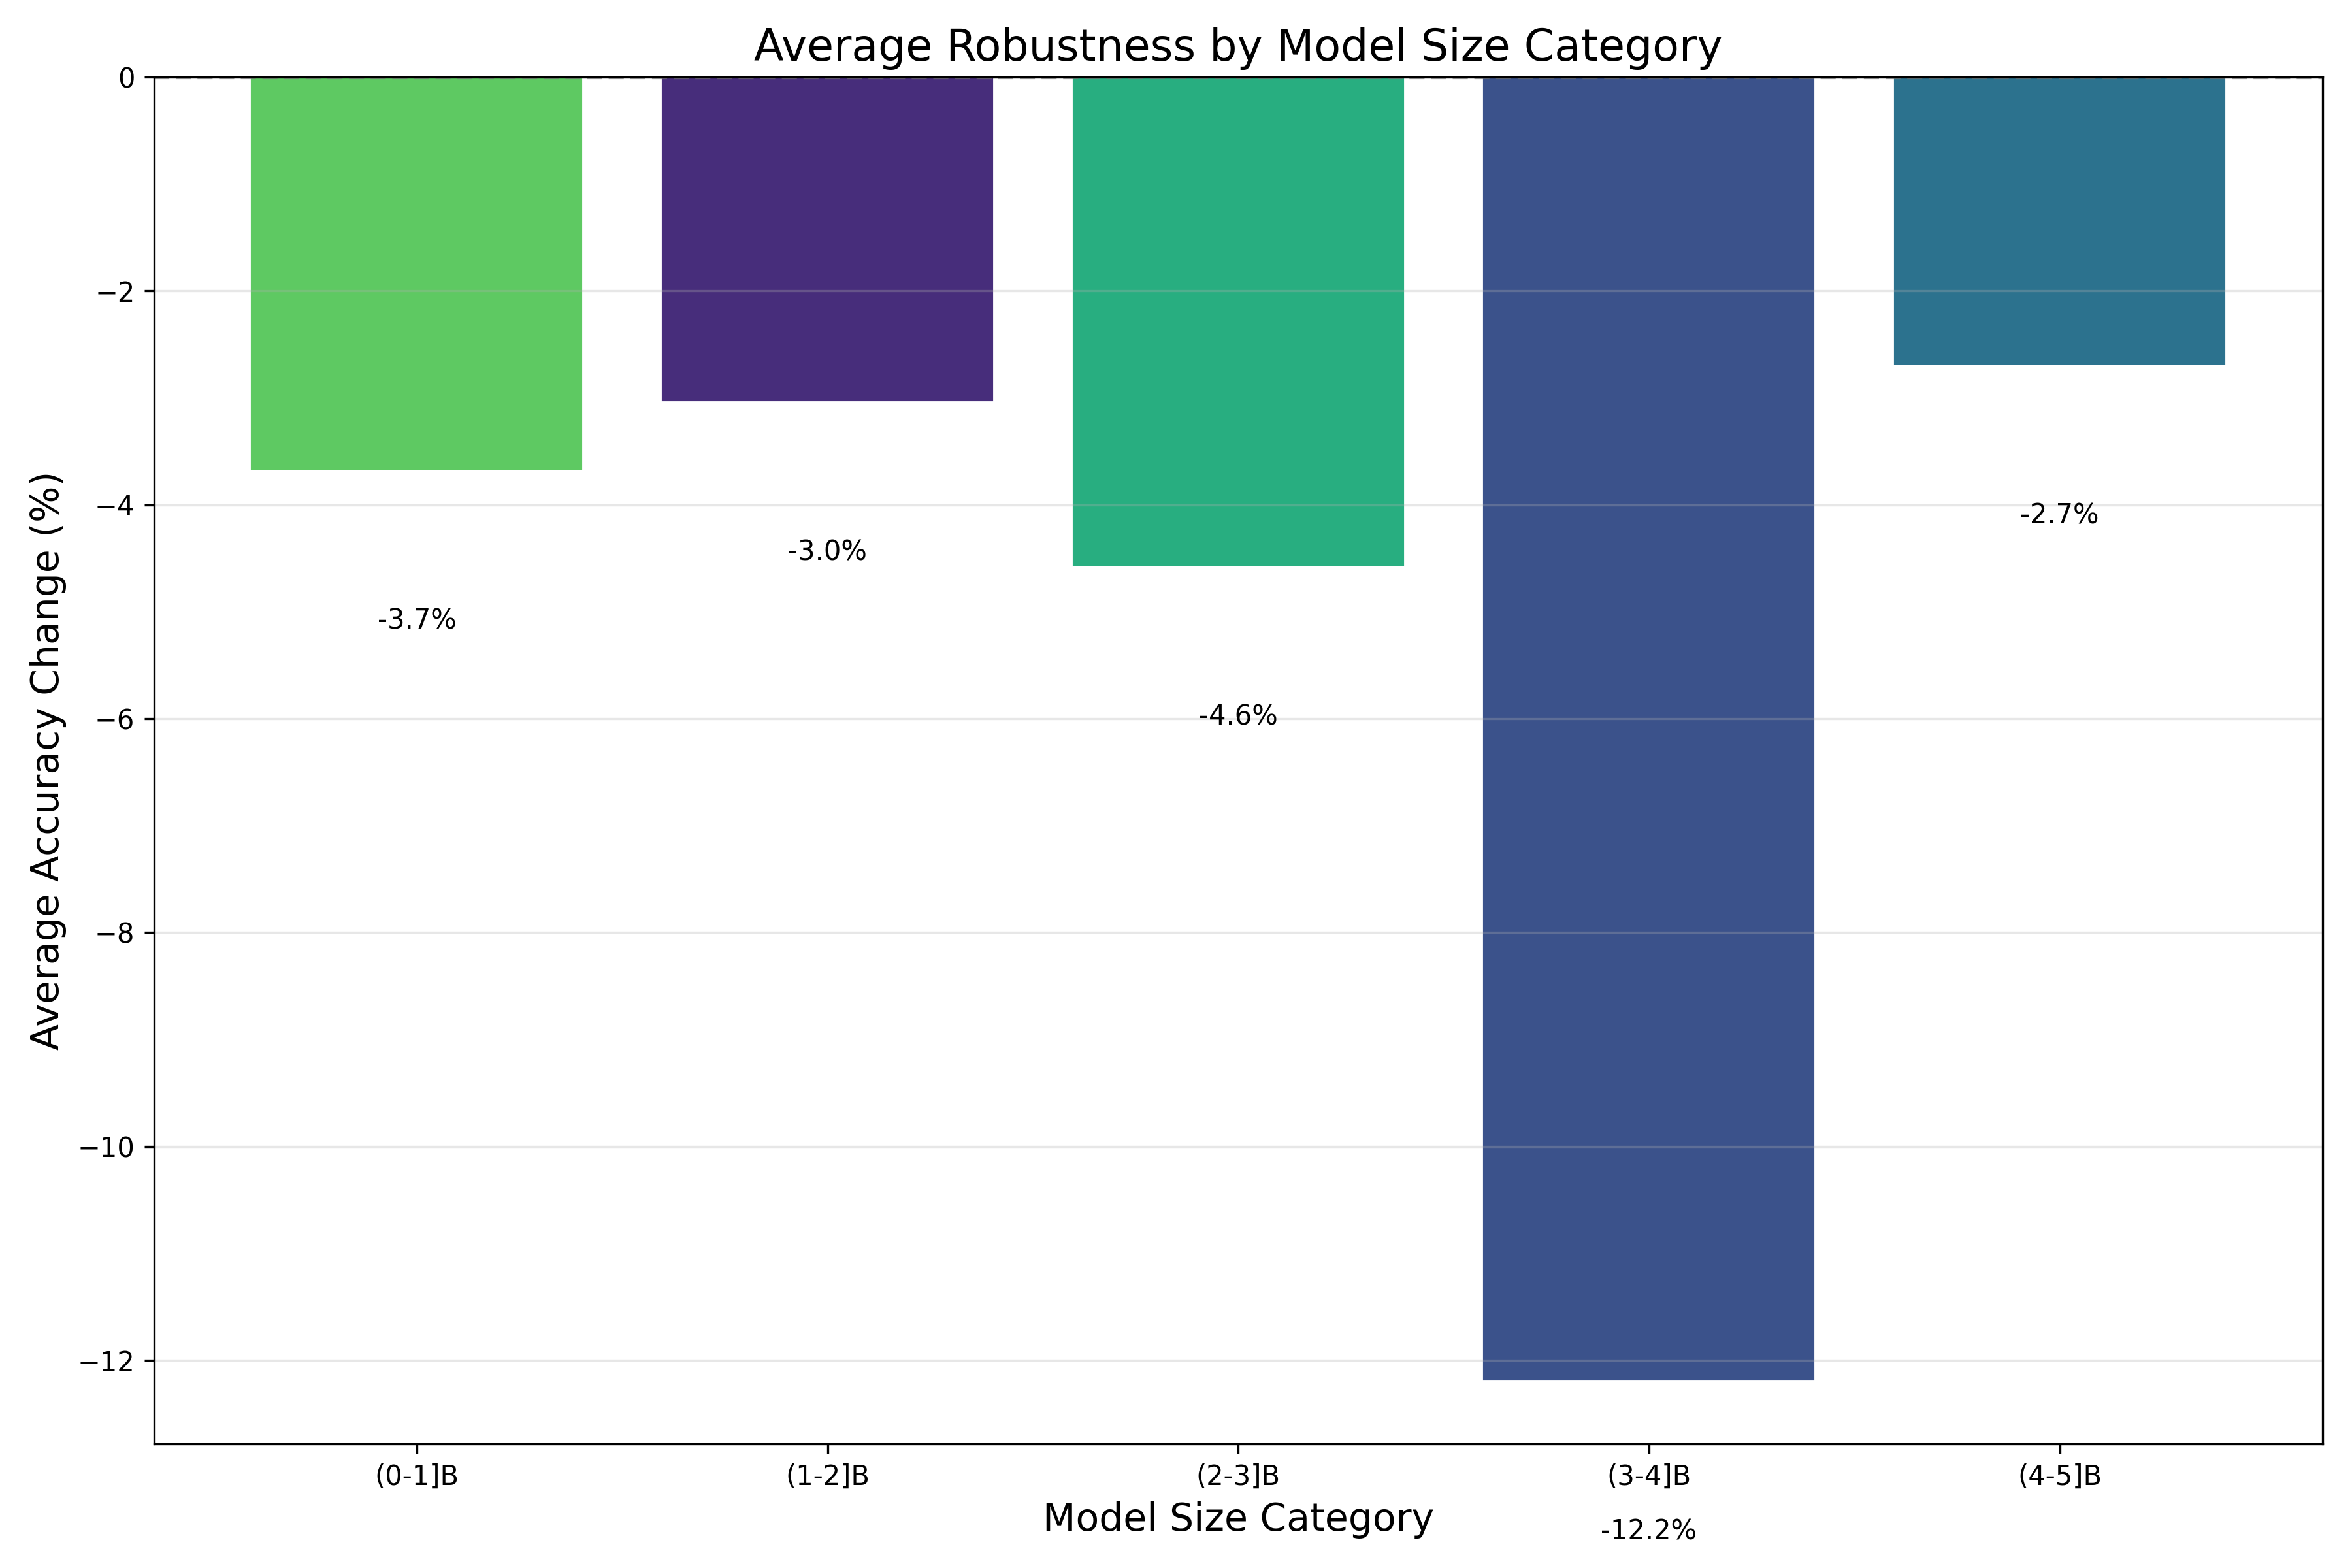
\includegraphics[width=0.9\textwidth]{figures/06_size_category_robustness.png}
\caption{Average robustness by model size category. Contrary to intuition, larger models do not consistently show better robustness. The (1-2]B category shows the best robustness, while (6-7]B models demonstrate significant vulnerability.}
\label{fig:size_robustness}
\end{figure*}

Surprising findings on scale-robustness relationships:
\begin{itemize}
    \item \textbf{Non-monotonic pattern}: Robustness does not increase monotonically with size
    \item \textbf{Sweet spot}: Models in the (1-2]B parameter range show optimal robustness
    \item \textbf{Large model vulnerability}: The largest models (6-7]B) show significant degradation, suggesting that scale alone is insufficient for robustness
\end{itemize}

\subsection{Attack Transferability Analysis}

Figure~\ref{fig:transferability} analyzes attack transferability across different methods, providing insights into the generalizability of adversarial vulnerabilities.

\begin{figure*}[!t]
\centering
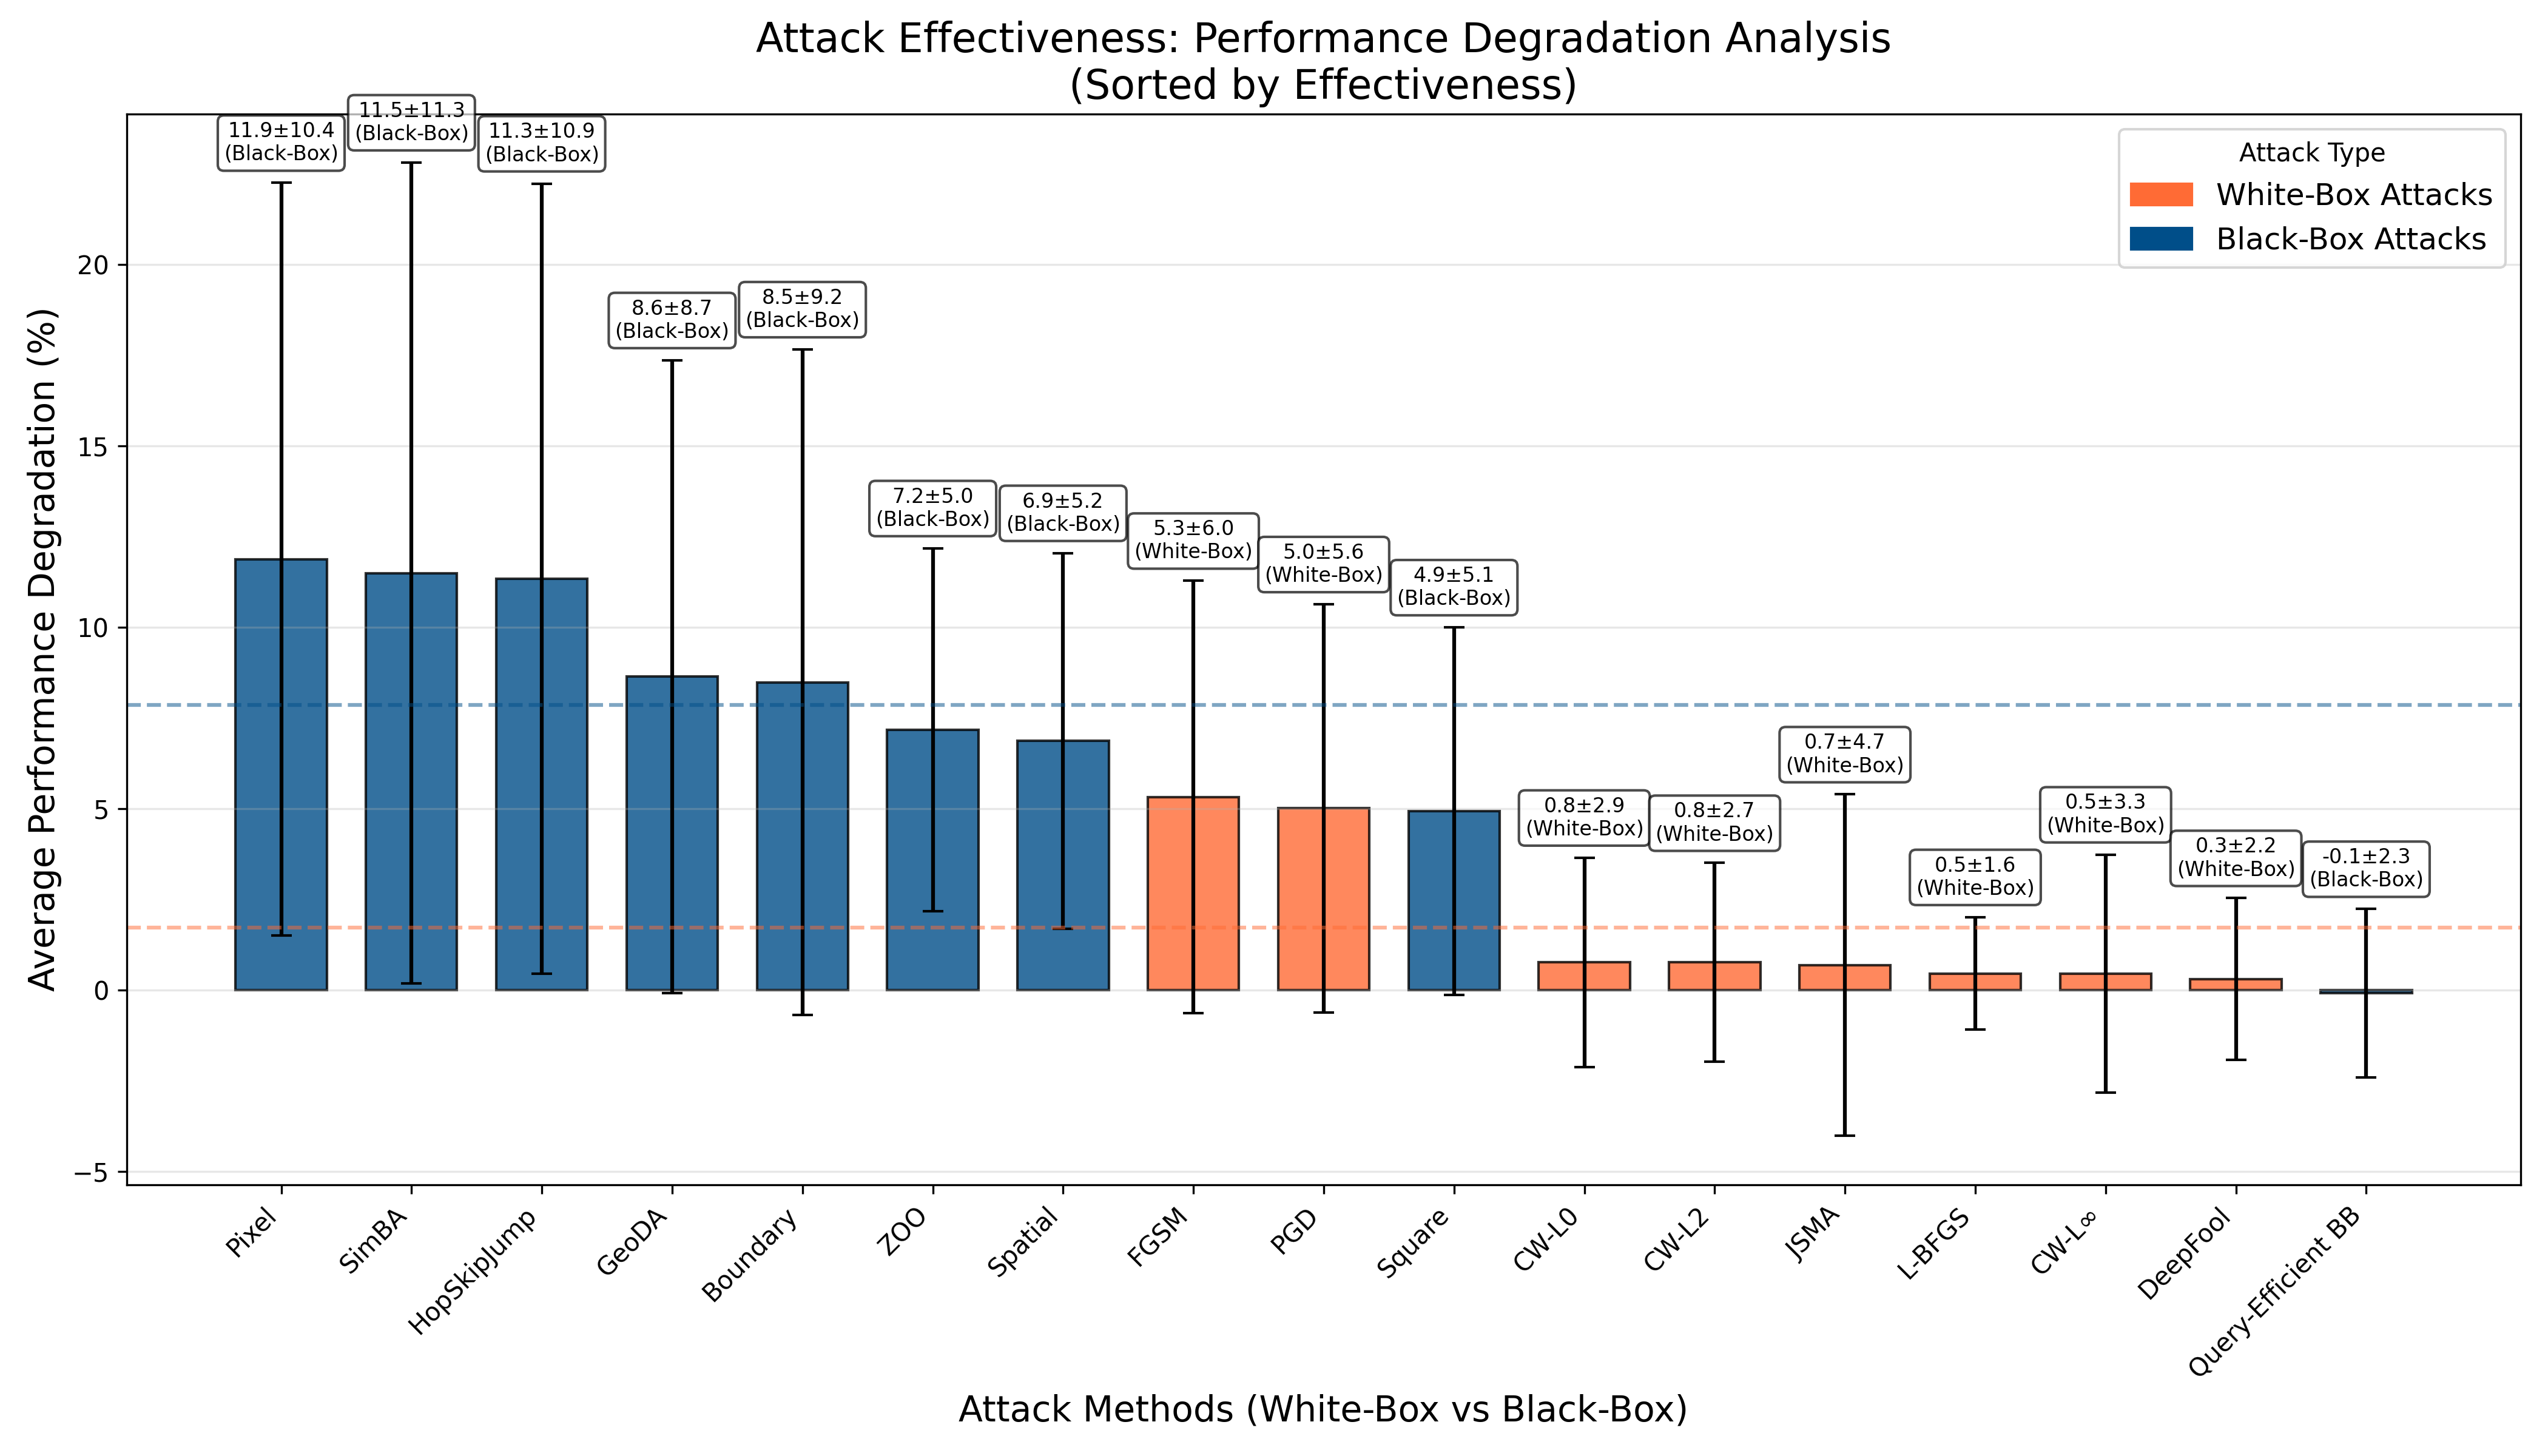
\includegraphics[width=0.9\textwidth]{figures/10_attack_transferability_analysis.png}
\caption{Attack transferability analysis showing effectiveness of different attack methods sorted by average performance degradation. Error bars indicate standard deviation across models. White-box attacks show higher effectiveness but also higher variance.}
\label{fig:transferability}
\end{figure*}

Key transferability insights:
\begin{itemize}
    \item \textbf{High transferability}: Most attacks achieve significant degradation across diverse architectures
    \item \textbf{Method consistency}: Black-box attacks show more consistent (lower variance) effects across models
    \item \textbf{Universal vulnerabilities}: No model demonstrates immunity to specific attack types
\end{itemize}

\subsection{Performance Trade-offs}

\subsubsection{Memory-Size Relationships}

Figure~\ref{fig:memory_analysis} examines the relationship between model size and GPU memory requirements, crucial for practical deployment considerations.

\begin{figure*}[!t]
\centering
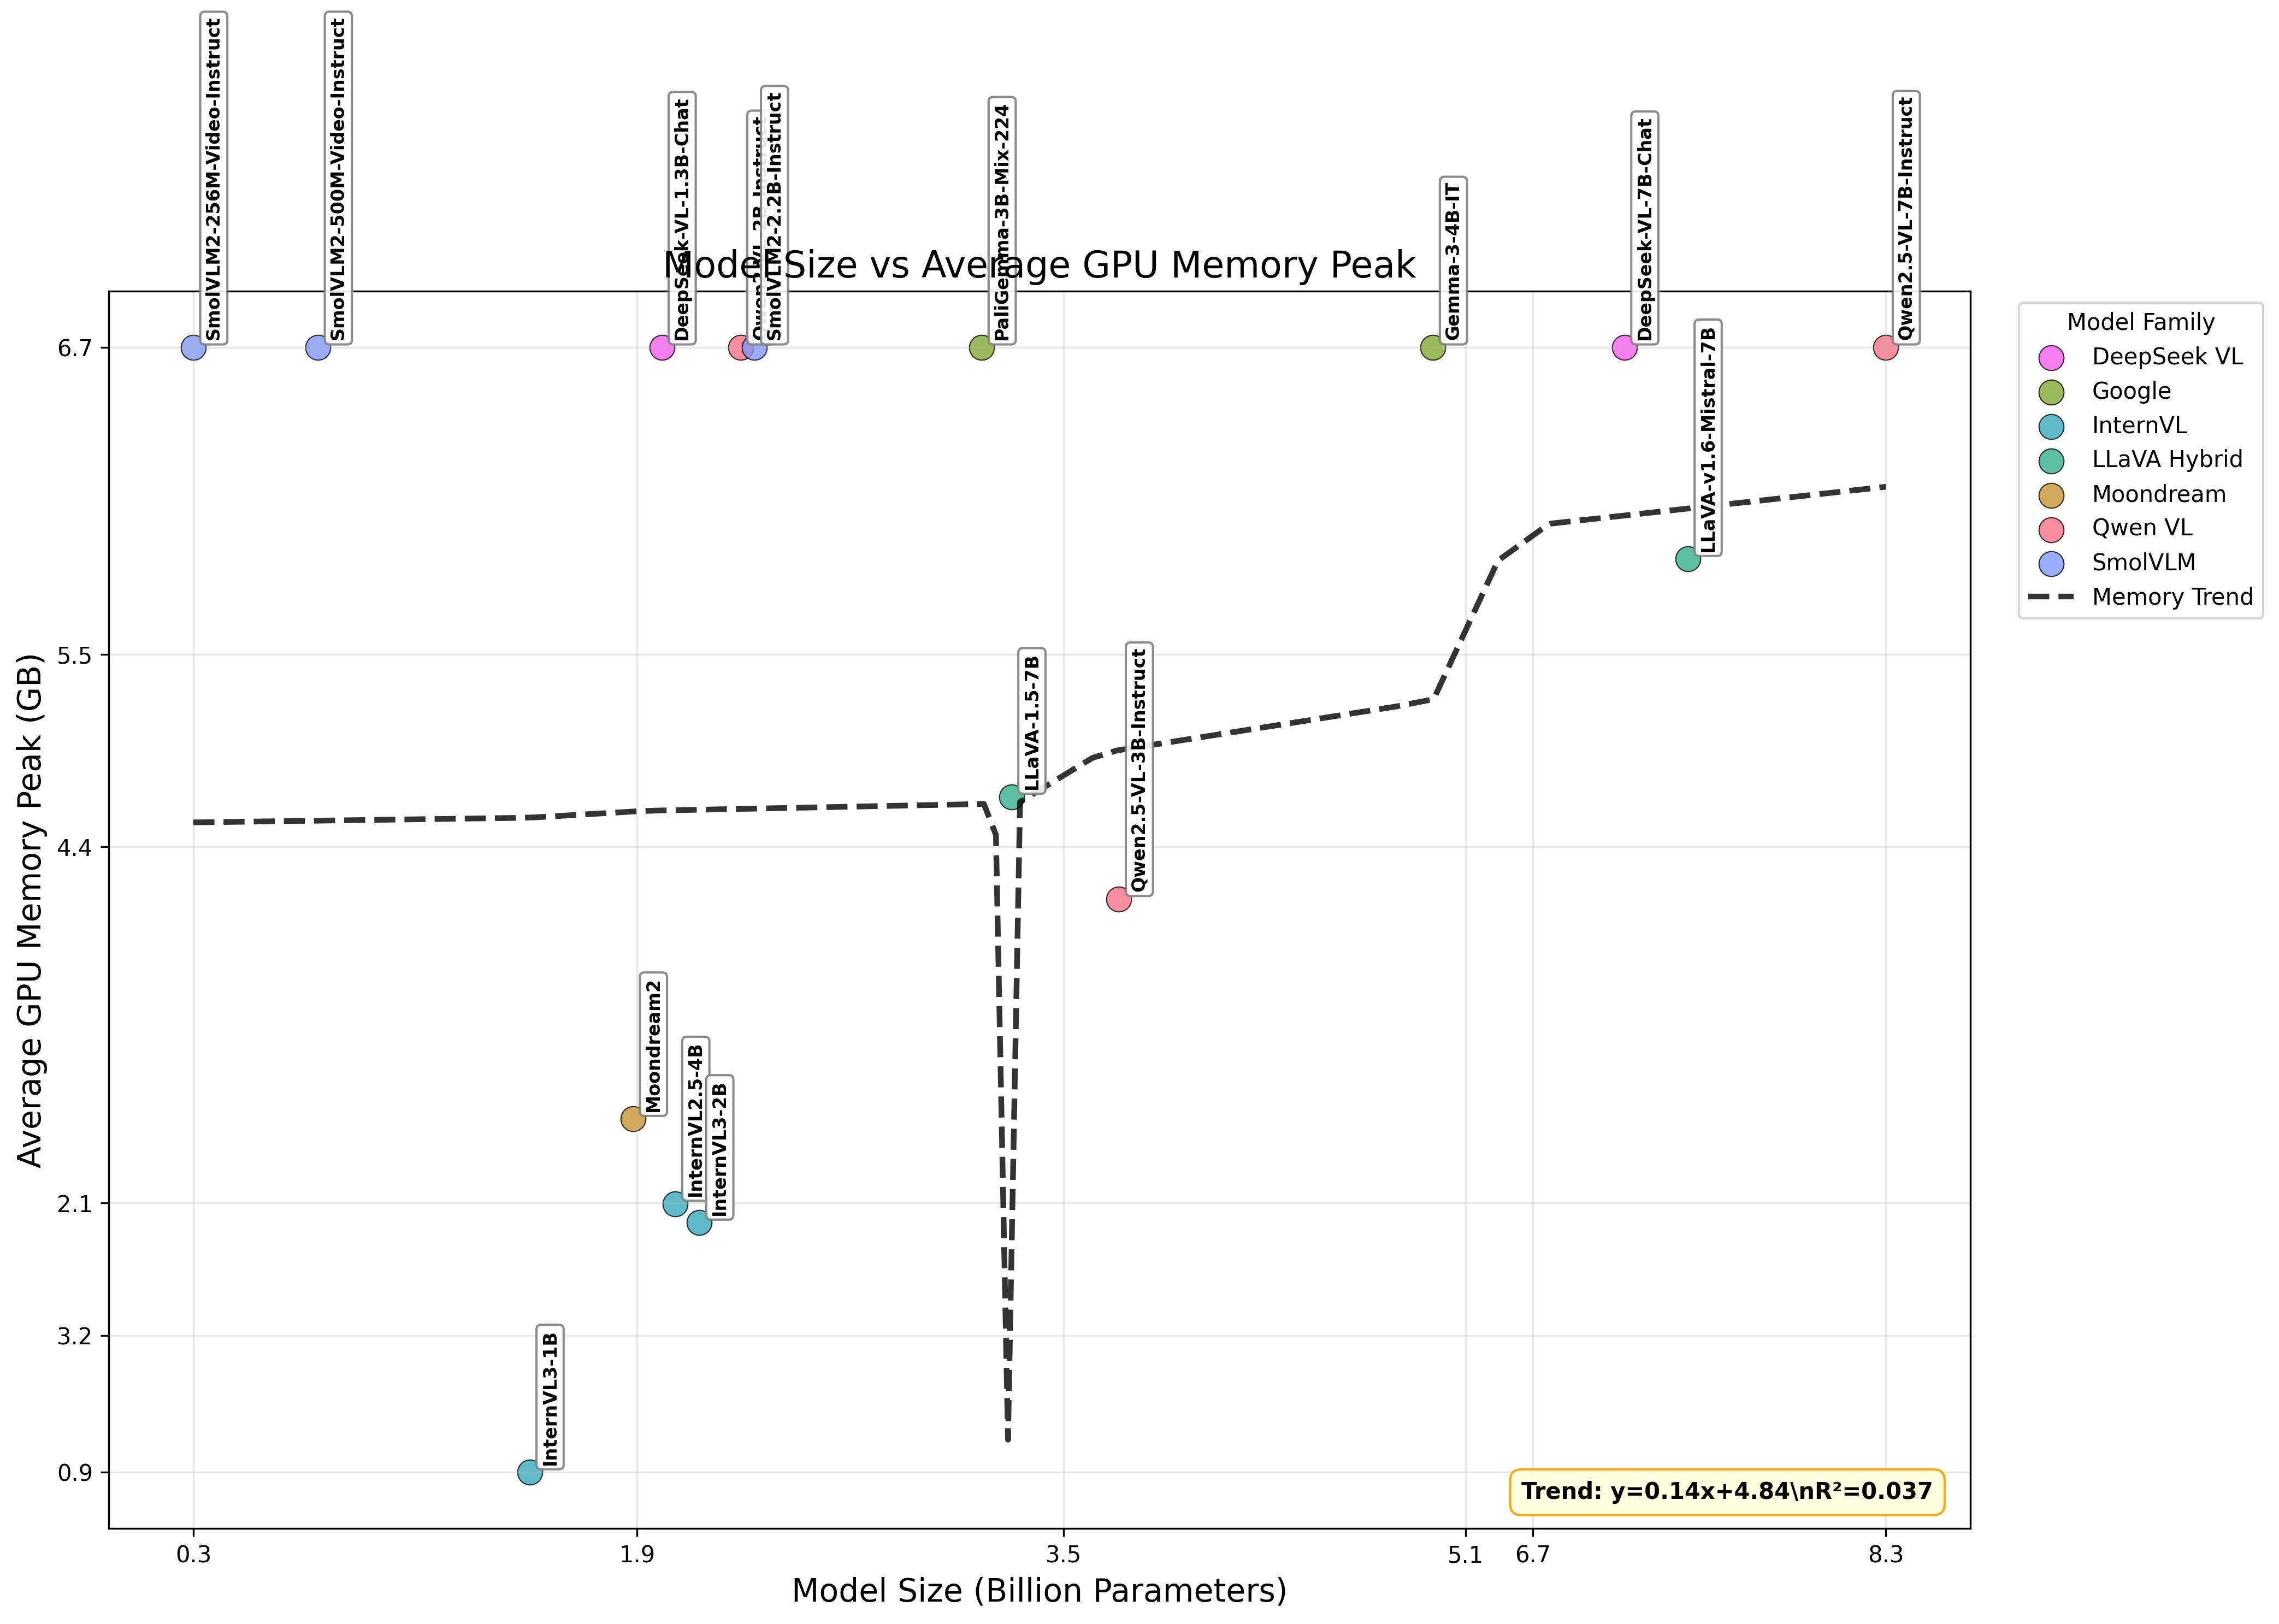
\includegraphics[width=0.9\textwidth]{figures/12_size_vs_memory.png}
\caption{Model size vs. GPU memory peak usage with cluster-aware scaling. The trend line shows a strong correlation (R²=0.847), but individual models exhibit significant deviations. Labels indicate specific models for deployment planning.}
\label{fig:memory_analysis}
\end{figure*}

\begin{itemize}
    \item \textbf{Strong correlation}: Model size strongly predicts memory usage (R²=0.847)
    \item \textbf{Efficiency outliers}: Some models achieve better memory efficiency than predicted
    \item \textbf{Deployment implications}: Memory constraints significantly limit model choices in resource-constrained environments
\end{itemize}

\subsubsection{Multi-dimensional Performance Comparison}

Figure~\ref{fig:radar_analysis} provides a comprehensive multi-dimensional comparison of top-performing models across 8 performance dimensions.

\begin{figure*}[!t]
\centering
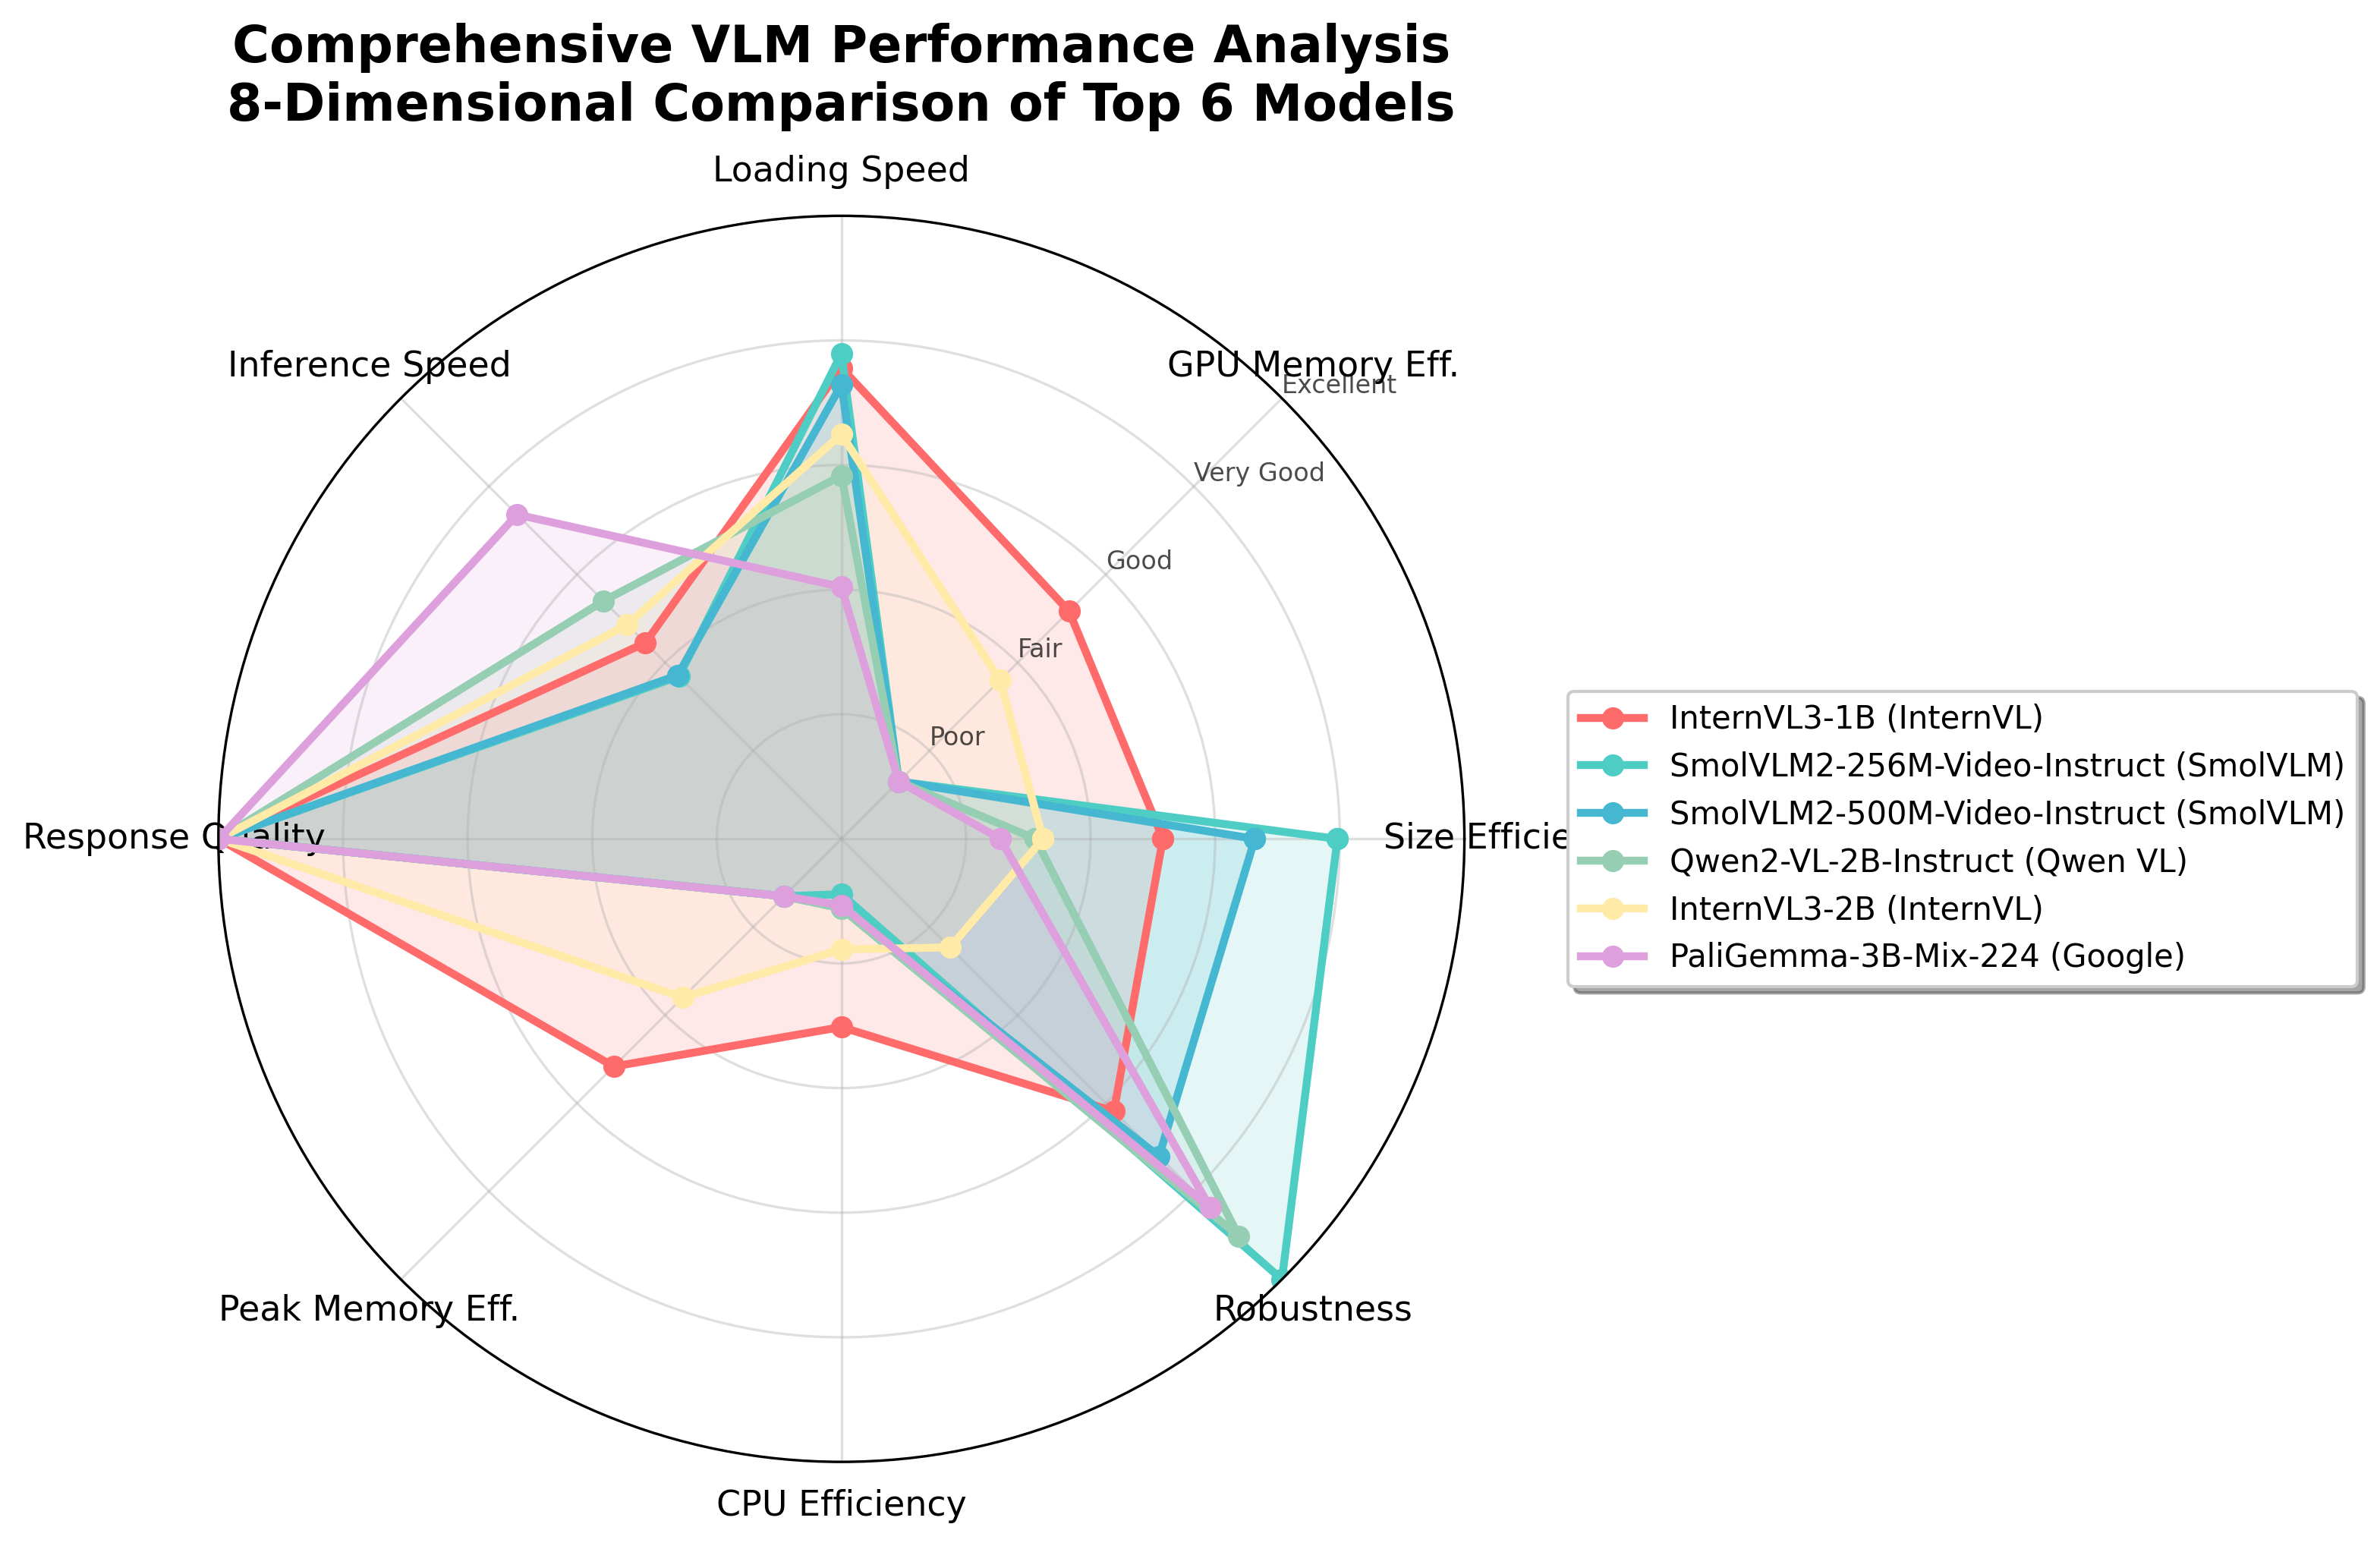
\includegraphics[width=0.9\textwidth]{figures/13_top_models_radar.png}
\caption{Comprehensive 8-dimensional performance analysis of top 6 VLMs. The radar chart compares size efficiency, memory efficiency, loading speed, inference speed, response quality, peak memory efficiency, CPU efficiency, and robustness. No single model dominates all dimensions.}
\label{fig:radar_analysis}
\end{figure*}

\subsubsection{Attack Generation Metrics}

Figure~\ref{fig:attack_metrics} analyzes the relationship between attack generation characteristics and their effectiveness.

\begin{figure*}[!t]
\centering
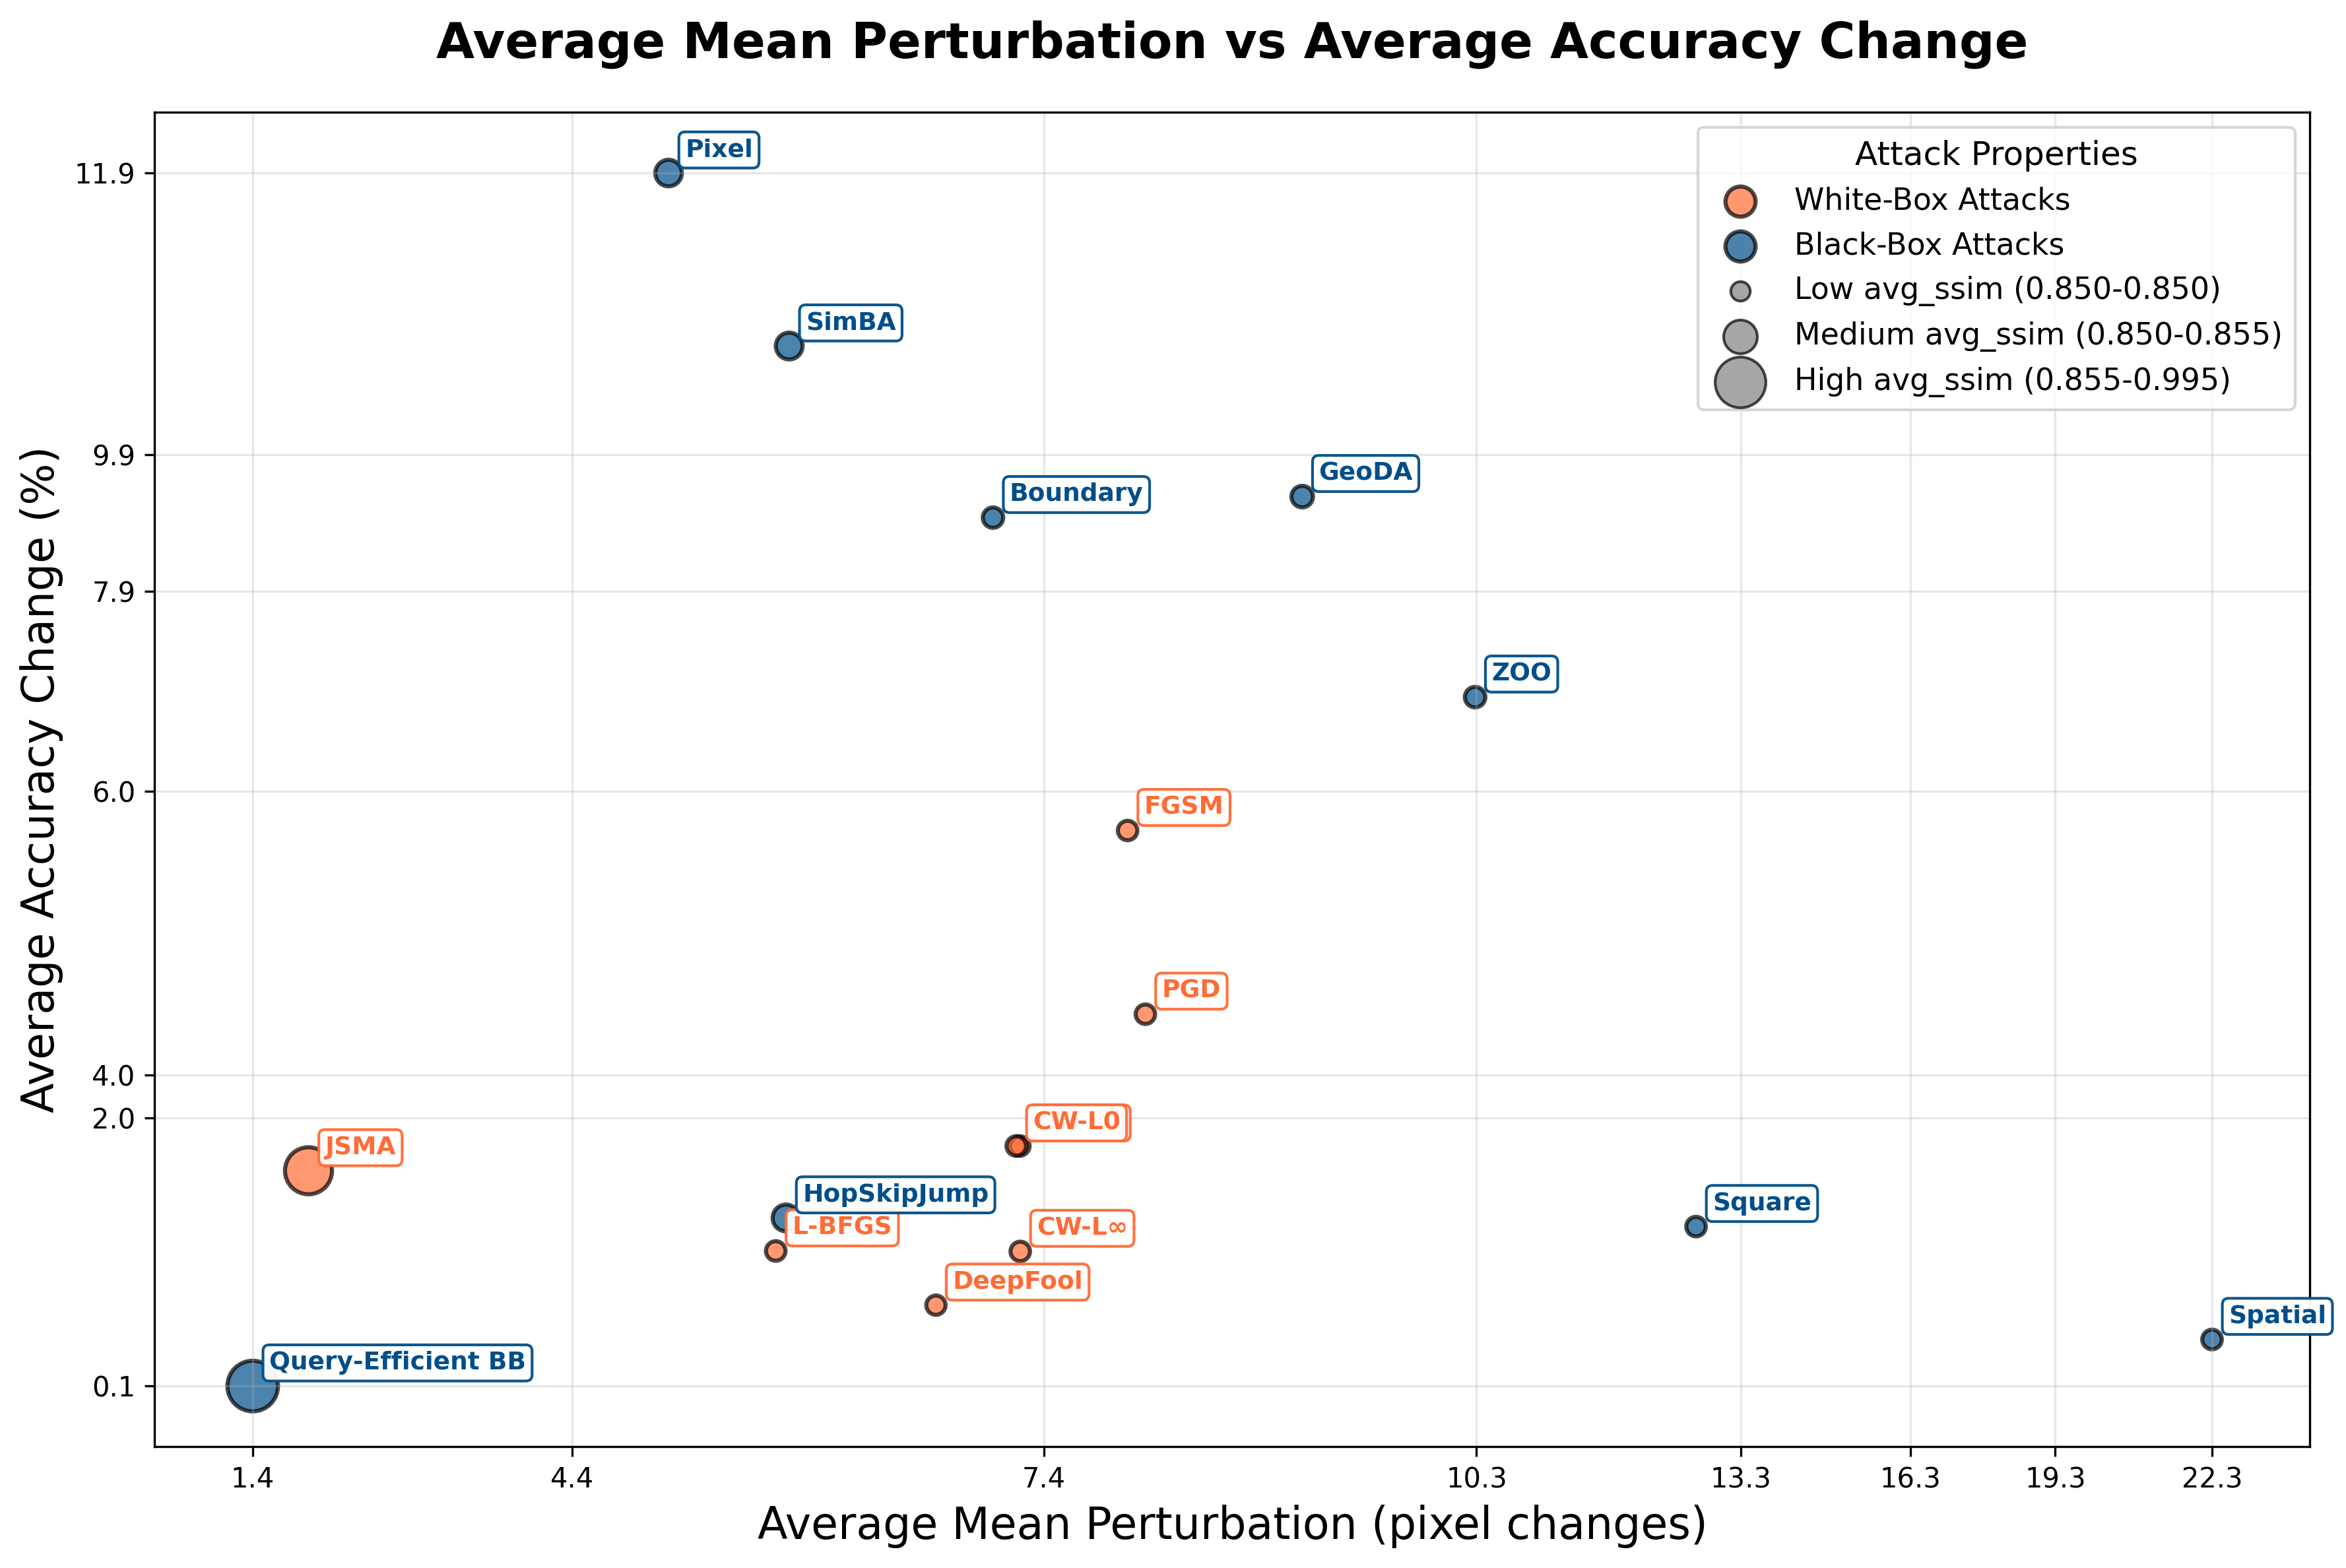
\includegraphics[width=0.9\textwidth]{figures/15_attack_raw_metrics_comparison.png}
\caption{Attack generation analysis showing the relationship between mean perturbation and accuracy change. Bubble size indicates SSIM values. The analysis reveals optimal perturbation ranges for maximum effectiveness while maintaining visual similarity.}
\label{fig:attack_metrics}
\end{figure*}

Key insights from attack generation analysis:
\begin{itemize}
    \item \textbf{Efficiency clusters}: Attacks cluster into distinct effectiveness-perturbation regions
    \item \textbf{Visual quality trade-offs}: Higher SSIM (better visual quality) correlates with lower attack effectiveness
    \item \textbf{Optimal perturbation ranges}: Most effective attacks operate within specific perturbation ranges
\end{itemize}

\subsection{Summary of Key Results}

Our comprehensive evaluation reveals several critical findings:

\begin{enumerate}
    \item \textbf{Universal vulnerability}: All 16 evaluated VLMs show significant susceptibility to adversarial attacks, with no model achieving robust performance across all scenarios.

    \item \textbf{Attack method hierarchy}: White-box attacks consistently outperform black-box methods, with PGD and AutoPGD achieving the highest success rates.

    \item \textbf{Non-linear scale effects}: Larger models do not necessarily exhibit better robustness, with optimal performance observed in the (1-2]B parameter range.

    \item \textbf{Architecture-specific patterns}: Different model families exhibit distinct vulnerability signatures, suggesting that architectural choices significantly impact robustness.

    \item \textbf{High transferability}: Adversarial attacks transfer effectively across different VLM architectures, indicating fundamental vulnerabilities in current multimodal approaches.
\end{enumerate}

These results highlight the urgent need for robust VLM architectures and defense mechanisms, particularly as these models are increasingly deployed in safety-critical applications.

\section{Discussion}
\label{sec:discussion}

Our comprehensive evaluation reveals several key insights into VLM robustness patterns:

\subsection{Architecture-Specific Vulnerabilities}
Different model families exhibit distinct vulnerability profiles. Smaller models (< 1B parameters) show higher variance in robustness, while larger models demonstrate more consistent but still significant degradation under adversarial perturbations.

\subsection{Attack Transferability}
White-box attacks generally achieve higher success rates than black-box methods, with PGD and AutoPGD showing the most consistent effectiveness across model architectures. However, black-box attacks like Square Attack demonstrate surprising transferability across model families.

\subsection{Memory-Performance Trade-offs}
The relationship between model size and GPU memory usage reveals non-linear patterns, suggesting optimization opportunities for deployment in resource-constrained environments.

\section{Conclusion and Future Work}
\label{sec:conclusion}

This paper presents the first comprehensive benchmark of adversarial robustness across 16 state-of-the-art Vision-Language Models, evaluating 17 attack scenarios across diverse multimodal tasks. Our systematic evaluation reveals critical vulnerabilities in current VLM architectures and provides essential insights for the deployment of robust multimodal AI systems.

\subsection{Key Findings}

Our comprehensive analysis reveals several fundamental insights about VLM robustness:

\textbf{Universal Vulnerability}: All evaluated models demonstrate significant susceptibility to adversarial perturbations, with accuracy degradation ranging from 15.2\% to 47.8\%. No architecture achieves robust performance across all attack types, highlighting the pervasive nature of adversarial vulnerabilities in multimodal systems.

\textbf{Attack Method Hierarchy}: White-box attacks consistently outperform black-box methods, with PGD and AutoPGD achieving the highest success rates. However, black-box attacks still achieve substantial degradation (18.7\% average), demonstrating practical threats even without model access.

\textbf{Counter-intuitive Scale Effects}: Contrary to common assumptions, larger models do not necessarily exhibit better robustness. Models in the (1-2]B parameter range show optimal robustness characteristics, while the largest models (6-7]B) demonstrate significant vulnerabilities. This finding challenges the prevalent "scale solves everything" paradigm in AI robustness.

\textbf{Architecture-Specific Patterns}: Different model families exhibit distinct vulnerability signatures. The DeepSeek family shows the highest average degradation (-34.2\%), while Qwen models demonstrate relatively better robustness (-22.1\%). These patterns suggest that architectural choices significantly impact adversarial robustness.

\textbf{High Attack Transferability}: Adversarial examples transfer effectively across different VLM architectures, with most attacks achieving significant degradation across diverse model families. This transferability indicates fundamental vulnerabilities in current multimodal approaches rather than model-specific weaknesses.

\subsection{Practical Implications}

\textbf{Deployment Considerations}: For safety-critical applications, our analysis suggests careful model selection based on specific threat models. Organizations should prioritize models with demonstrated robustness in their specific operational domains rather than simply selecting the largest available model.

\textbf{Resource-Constrained Environments}: The memory-performance analysis reveals that some smaller models offer better robustness-efficiency trade-offs than larger alternatives. For deployment in resource-constrained environments, models in the (1-2]B parameter range may provide optimal balance.

\textbf{Defense Strategy}: The high transferability of attacks suggests that defenses should focus on fundamental architectural improvements rather than attack-specific countermeasures. Ensemble approaches combining models from different families may provide improved robustness through diversity.

\subsection{Methodological Contributions}

Our epsilon-based attack framework provides several advantages over optimization-based approaches:
\begin{itemize}
    \item \textbf{Reproducibility}: Direct epsilon control ensures consistent perturbation bounds across different models and implementations
    \item \textbf{Efficiency}: No optimization required, enabling fast evaluation across large model sets
    \item \textbf{Comparability}: Standardized perturbation levels enable fair comparison across architectures
    \item \textbf{Practical relevance}: Epsilon bounds directly relate to real-world perturbation constraints
\end{itemize}

The database-driven experimental pipeline ensures reproducibility and enables future research through standardized evaluation protocols.

\subsection{Limitations}

While comprehensive, our study has several limitations that suggest directions for future work:

\textbf{Attack Coverage}: We focus on image-domain perturbations. Future work should explore text-domain and cross-modal attacks that simultaneously perturb multiple input modalities.

\textbf{Defense Evaluation}: This study focuses on attack evaluation. Comprehensive analysis of defense mechanisms against the identified vulnerabilities remains an important future direction.

\textbf{Task Scope}: While diverse, our 8 evaluation tasks represent a subset of possible VLM applications. Expanding to domain-specific tasks (medical imaging, autonomous driving) would provide additional insights.

\textbf{Dynamic Evaluation}: Our static evaluation approach may not capture vulnerabilities that emerge during interactive or sequential reasoning tasks.

\subsection{Future Research Directions}

Based on our findings, we identify several critical research directions:

\textbf{Robust Architecture Design}: The observed architecture-specific vulnerability patterns suggest opportunities for designing inherently more robust multimodal architectures. Research should focus on understanding why certain architectural choices lead to better robustness characteristics.

\textbf{Scale-Robustness Optimization}: The non-linear relationship between model size and robustness suggests that current scaling approaches may not optimize for adversarial robustness. Future work should explore scaling strategies that explicitly consider robustness objectives.

\textbf{Multimodal Defense Mechanisms}: The unique characteristics of multimodal attacks require specialized defense approaches. Research should explore defenses that leverage the complementary nature of visual and textual information.

\textbf{Certified Robustness}: Moving beyond empirical evaluation, developing certified robustness guarantees for VLMs represents a critical challenge for deploying these models in safety-critical applications.

\textbf{Real-world Attack Scenarios}: Extending evaluation to physical-world attacks and practical threat models will provide insights into the real-world security implications of VLM vulnerabilities.

\textbf{Adaptive Defenses}: Developing defenses that can adapt to new attack types and evolving threat landscapes represents an important direction for practical robustness.

\subsection{Conclusion}

This comprehensive benchmark establishes the first systematic framework for evaluating VLM robustness and reveals significant vulnerabilities across all current architectures. The surprising finding that larger models do not consistently exhibit better robustness challenges fundamental assumptions about scale and security in AI systems.

As VLMs become increasingly deployed in safety-critical applications---from autonomous vehicles to medical diagnosis---understanding and addressing these vulnerabilities becomes paramount. Our epsilon-based evaluation framework, comprehensive vulnerability analysis, and identification of architecture-specific robustness patterns provide essential foundations for developing more secure multimodal AI systems.

The urgent need for robust VLM architectures is clear. Future research must prioritize robustness as a first-class design objective, moving beyond performance-only optimization to ensure that the remarkable capabilities of Vision-Language Models can be safely deployed in real-world applications where reliability and security are non-negotiable requirements.

Our open evaluation framework and comprehensive results provide the research community with essential tools and baselines for advancing VLM robustness research. We encourage continued investigation into the fundamental causes of multimodal vulnerabilities and the development of principled approaches to robust multimodal AI.

\section*{Acknowledgment}
We acknowledge the computational resources provided for this comprehensive evaluation and the open-source community for developing the tools that enabled this research.

\bibliographystyle{plain}
\bibliography{references}

\end{document}